    \subsubsection{Recommendations for each aspect}
    \paragraph{How often the software is updated}
    \begin{figure}[H]
        \centering
        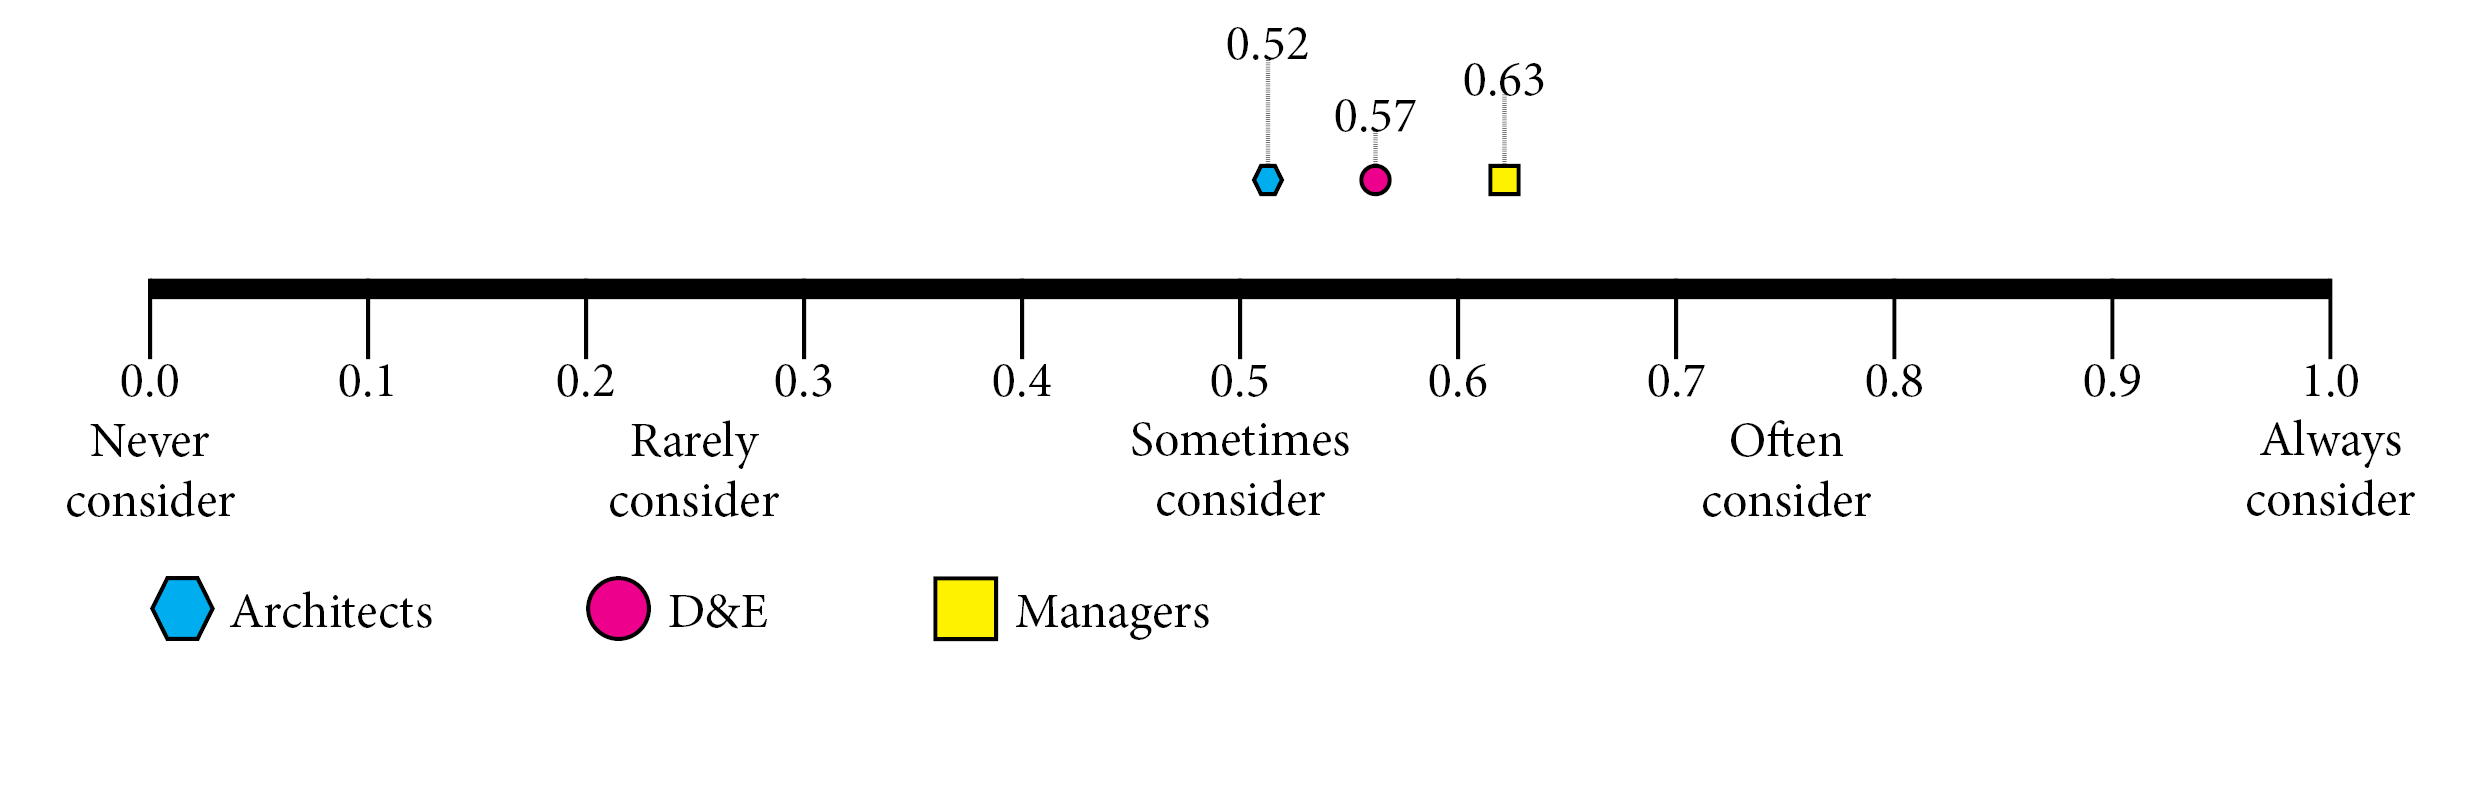
\includegraphics[width=\linewidth]{scorelines/aspect1.png}
        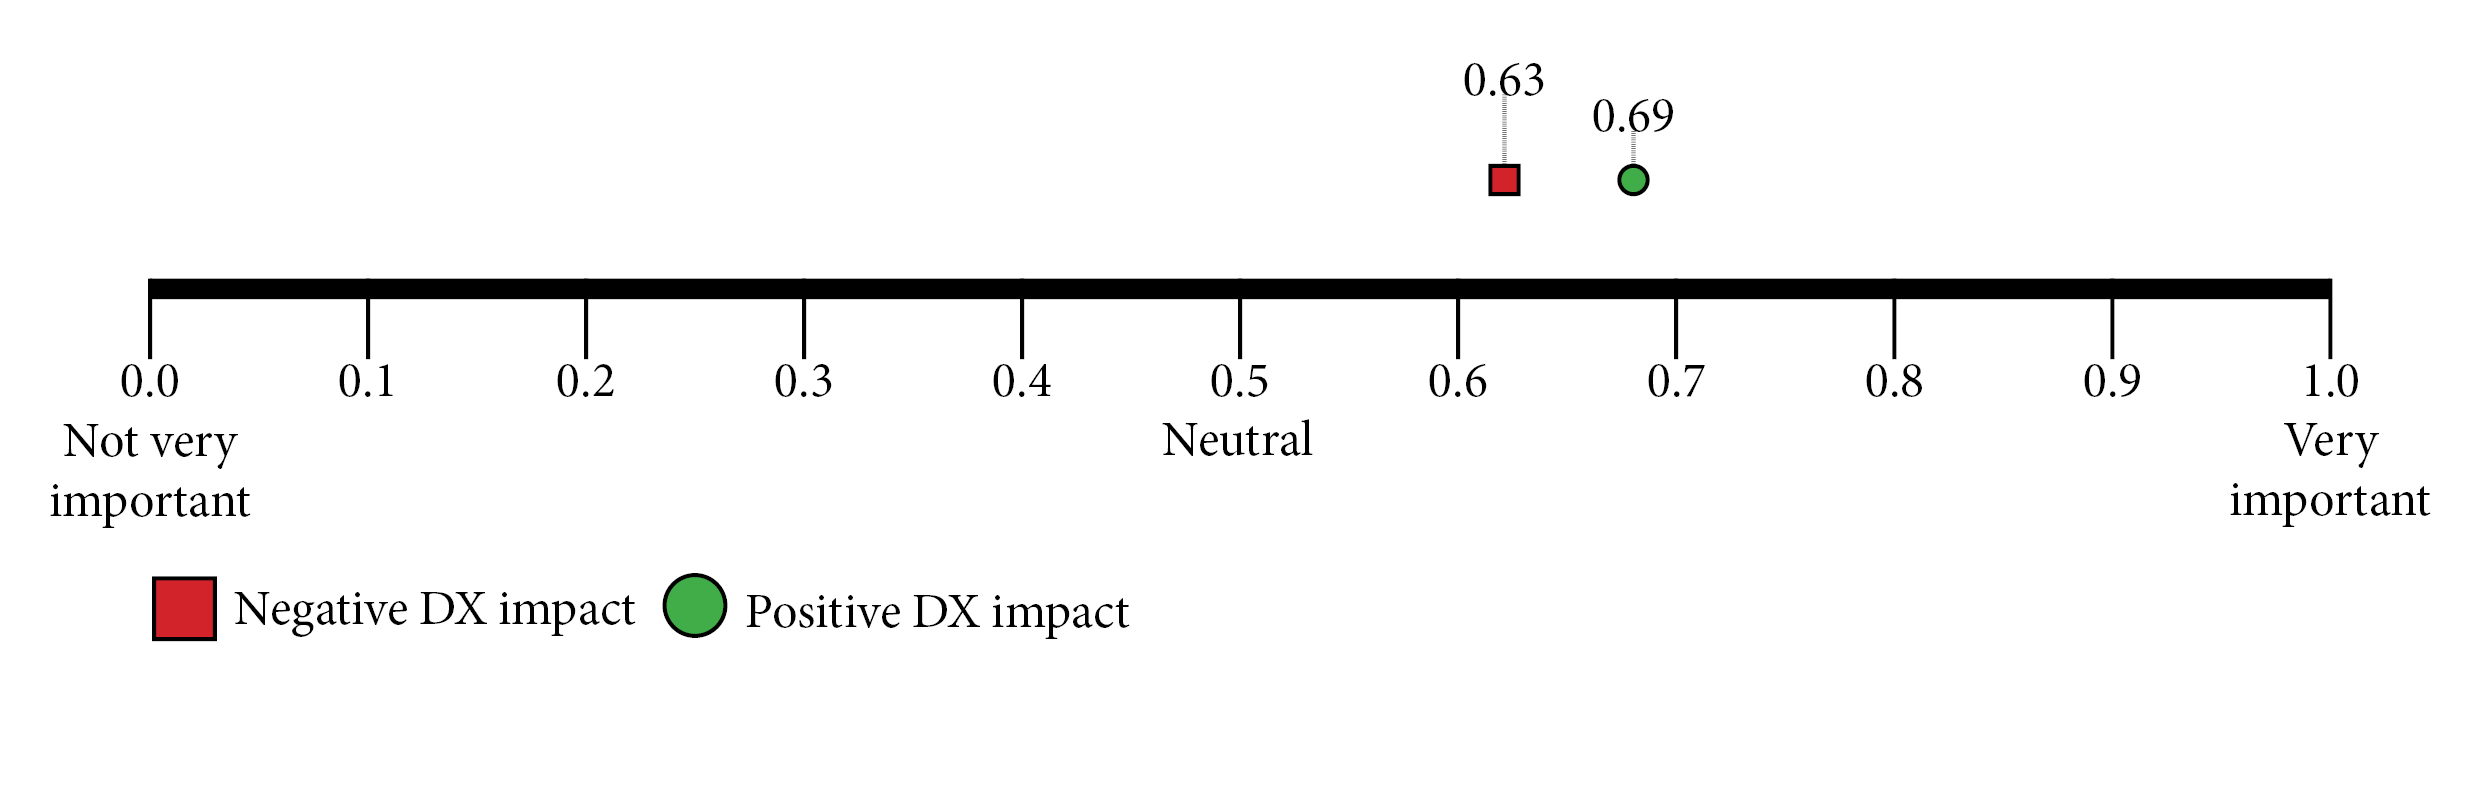
\includegraphics[width=\linewidth]{dxscorelines/dxaspect1.png}
        \caption{Scoring for "How often the software is updated"}
        \label{fig:aspect1}
    \end{figure}
    Updating of the software platform is of course important. Bugs need to be fixed, the compatibility for different platforms improved and new features might be added from time to time. In figure \ref{fig:aspect1} we can see how it's ranked. As we can see it's ranking somewhere in the middle. The interviews showed that how often the software is updated can be seen as an indicator for how mature the software platform is. Too often and it will scare people away, as it's an indicator that there is a lot of bugs or the software is mature. If the software is updated not often enough it's an indicator that the software platform feels abandoned or not prioritised. The recommendation is to plan your updates carefully, try to lump small updates together into bigger ones, as to not update too often. Exemptions from this is critical bug fixes, such as relating to security or breaking bugs. To make this kind of planning is not a big effort, and therefor worth it. With the average score of 0.58/1.00 this aspect needs to be kept in mind, but not central. If you cater to managers, this aspect needs to kept more in mind. \\ \\
    \textbf{Verdict: Somewhat important, but keep in mind. Medium effort, medium payoff.}
    \paragraph{I can have working code quickly}
    \begin{figure}[H]
        \centering
        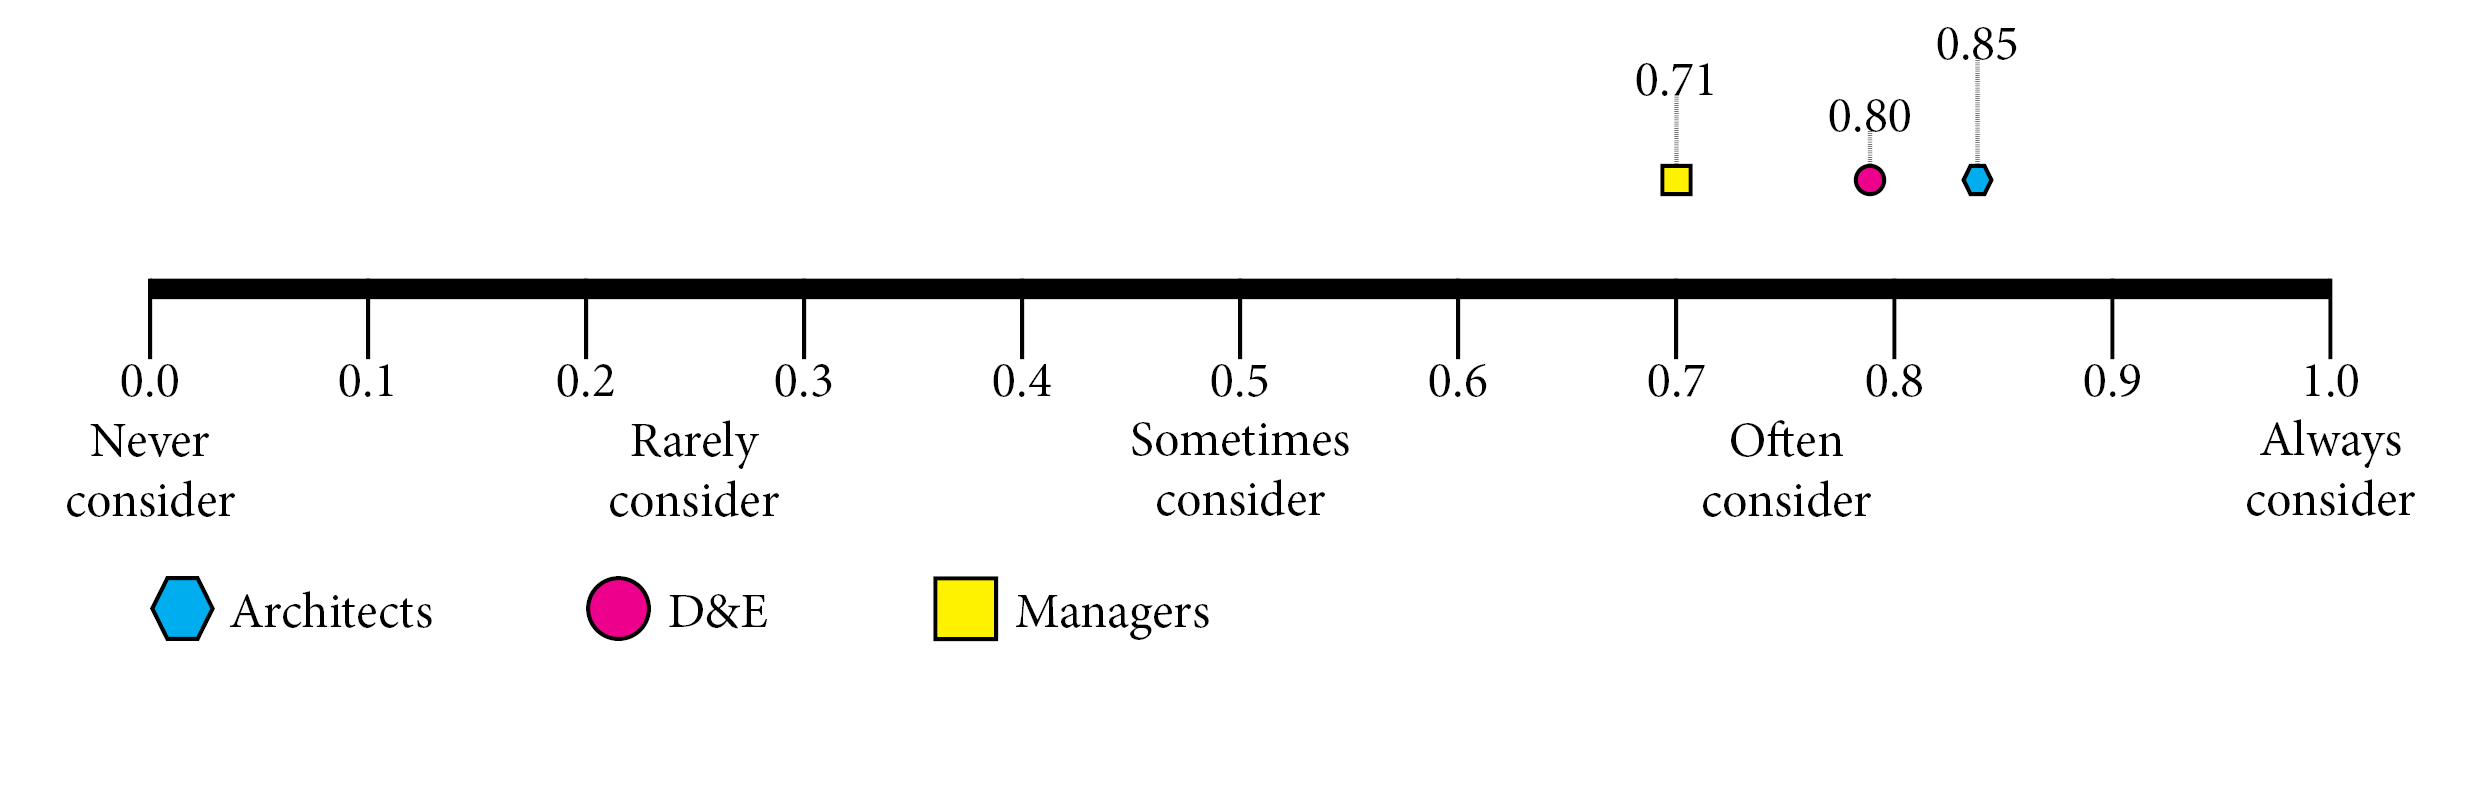
\includegraphics[width=\linewidth]{scorelines/aspect2.png}
        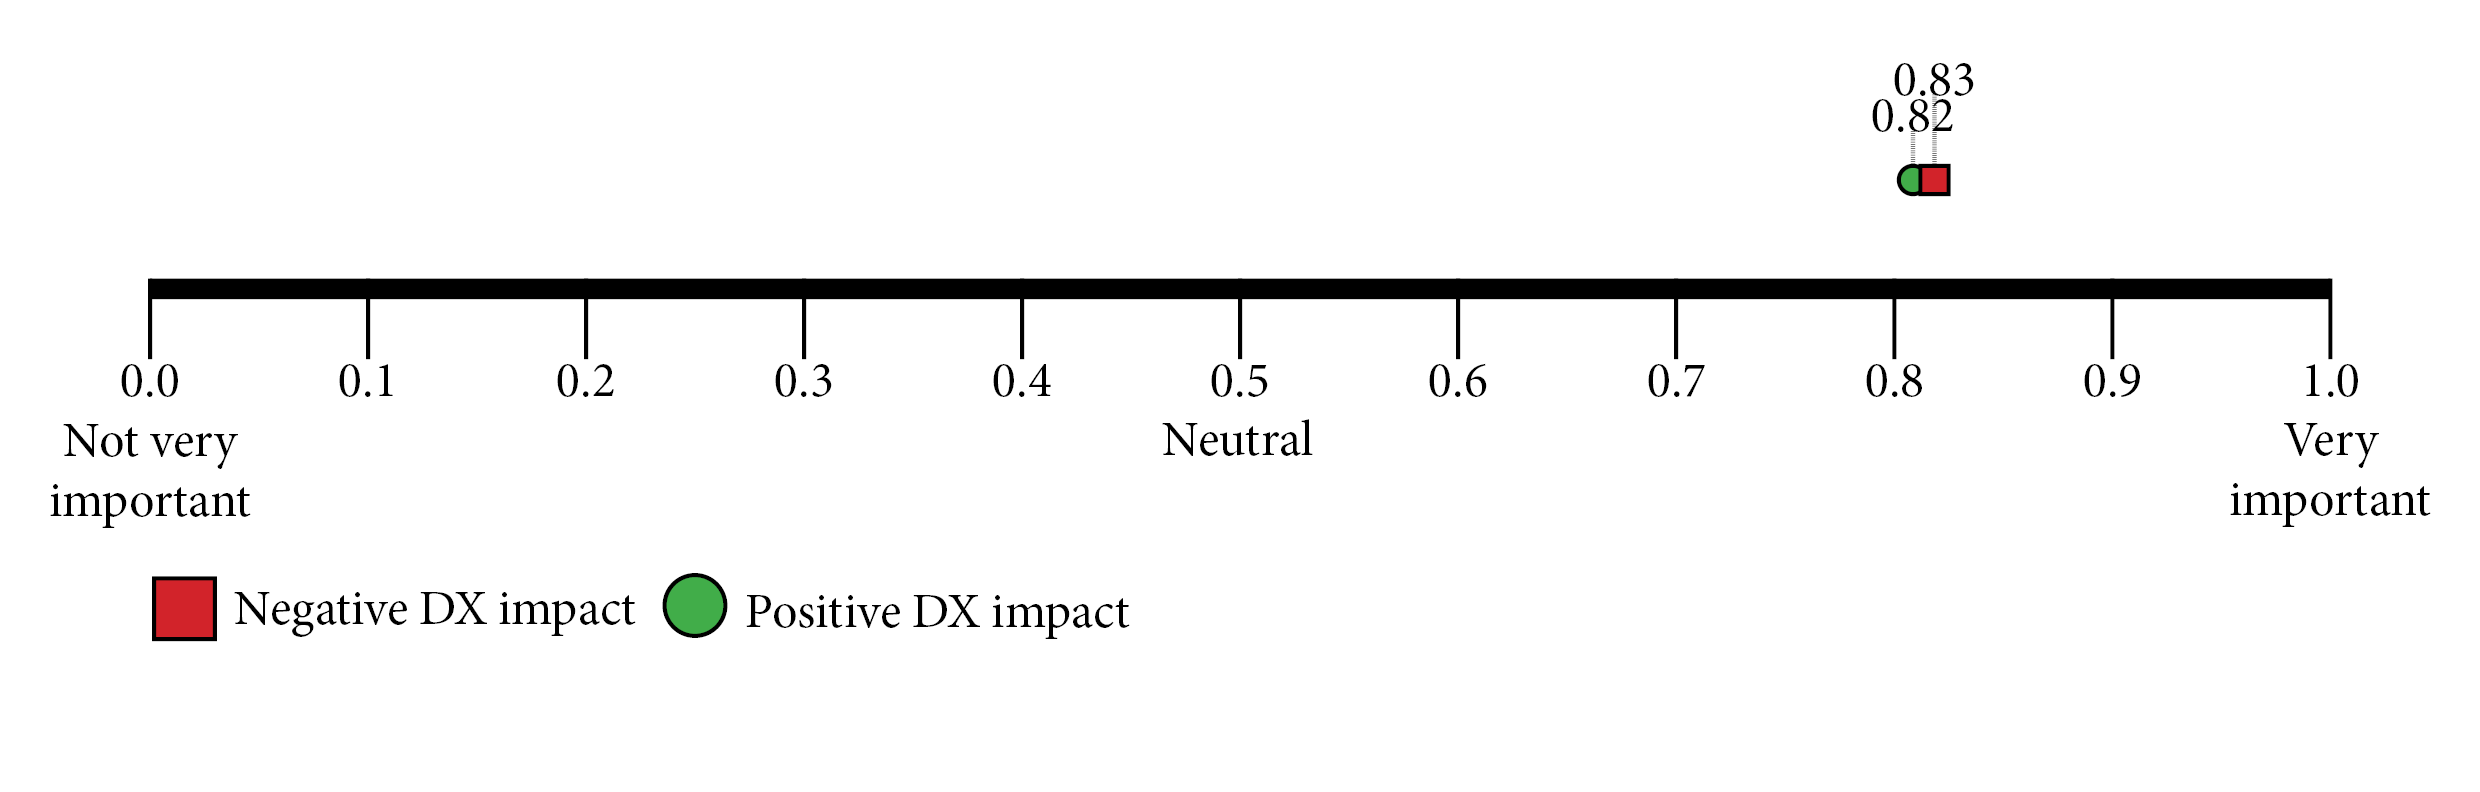
\includegraphics[width=\linewidth]{dxscorelines/dxaspect2.png}
        \caption{Scoring for "I can have working code quickly"}
        \label{fig:aspect2}
    \end{figure}
    Working code quickly has been shown to be important to developers. In figure \ref{fig:aspect2} we can see the scoring. With an average score of 0.80/1.00 this is an important aspect that should always be considered when creating a software platform. Not only are developers impatient people that want results quickly overall, working code quickly is developers way to figure out if a software platform is useful. Software developers quickly abandon software if they don't see it's value. Because working code quickly is their way of evaluating new software, it's extremely important to be able to provide this. The recommendation is to easily show how to get started. It should both be front and centre when you visit the website, and the example should be quick without being too simple. The effort to have an example that is easy to follow  and makes the user understand can take time, and be a bit of an effort, but is definitely worth it.\\ \\
    \textbf{Very important, always keep in mind. Medium effort, high payoff.}
    \paragraph{The API documentation gives thorough explanations on how it works}
    \begin{figure}[H]
        \centering
        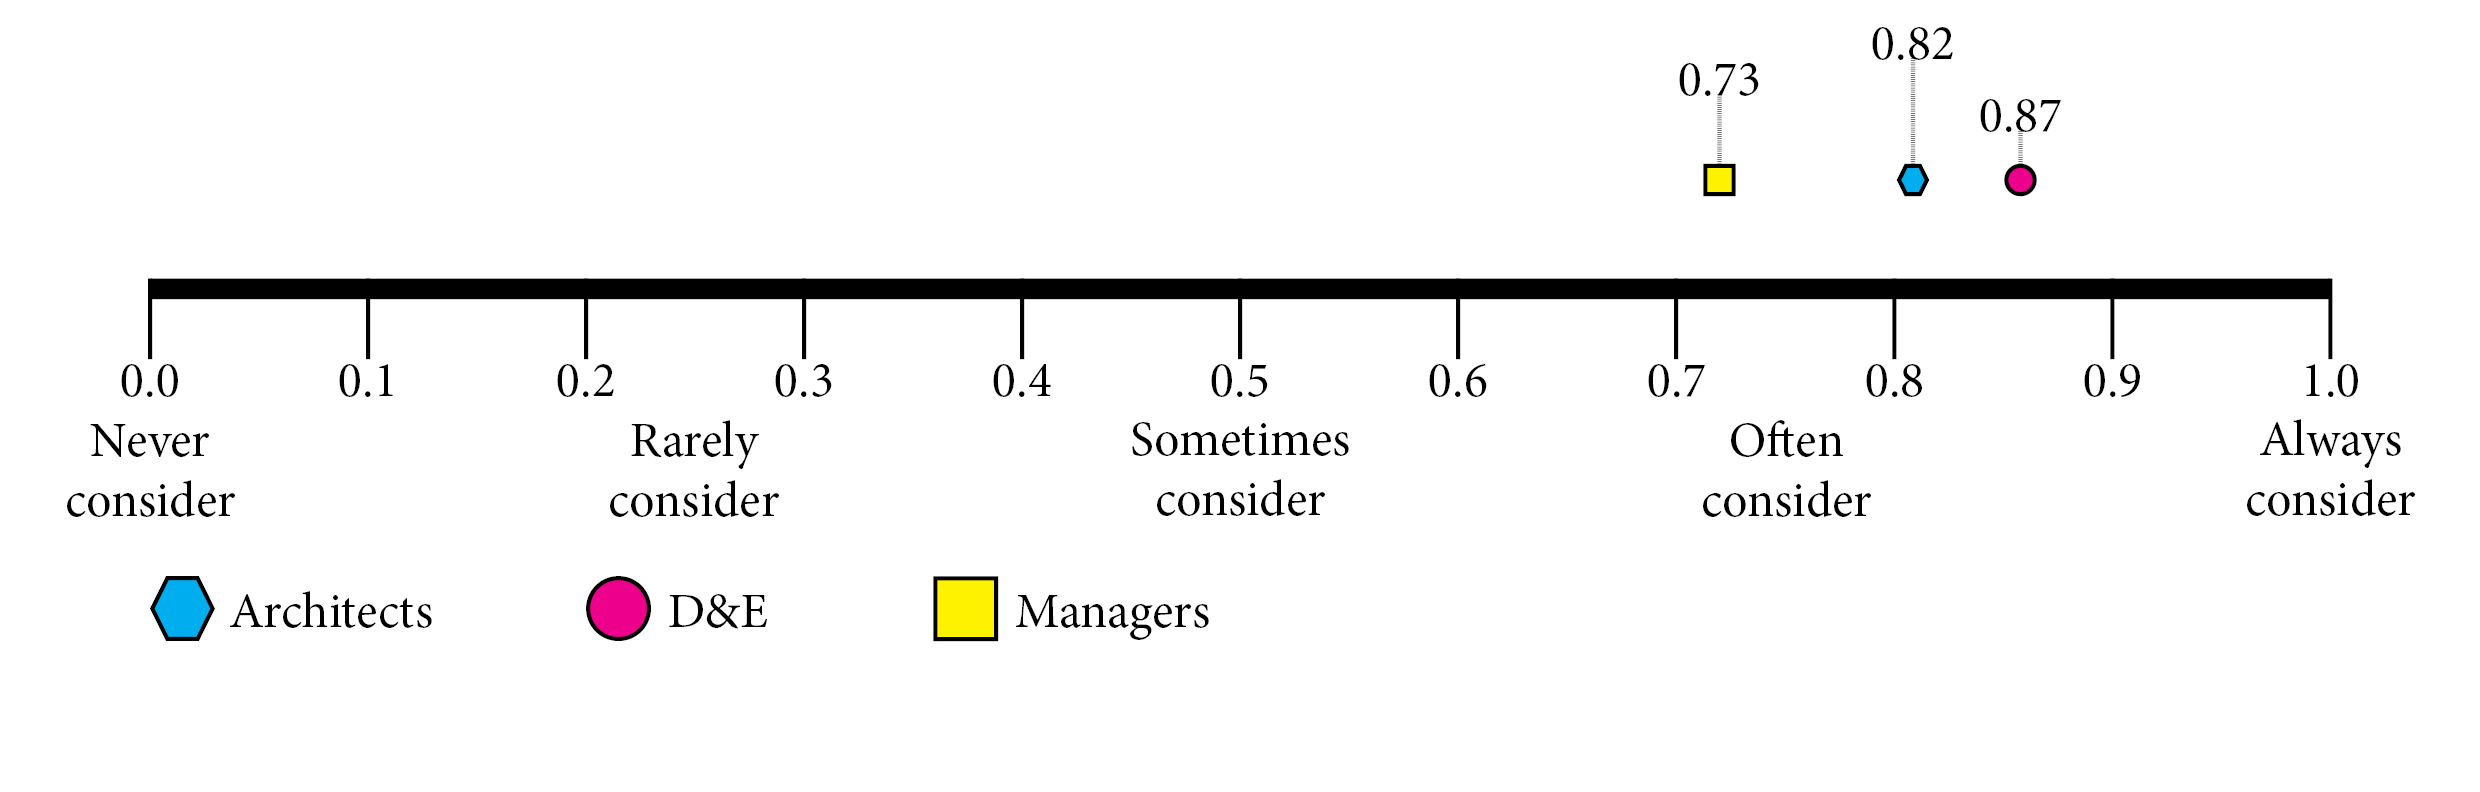
\includegraphics[width=\linewidth]{scorelines/aspect3.png}
        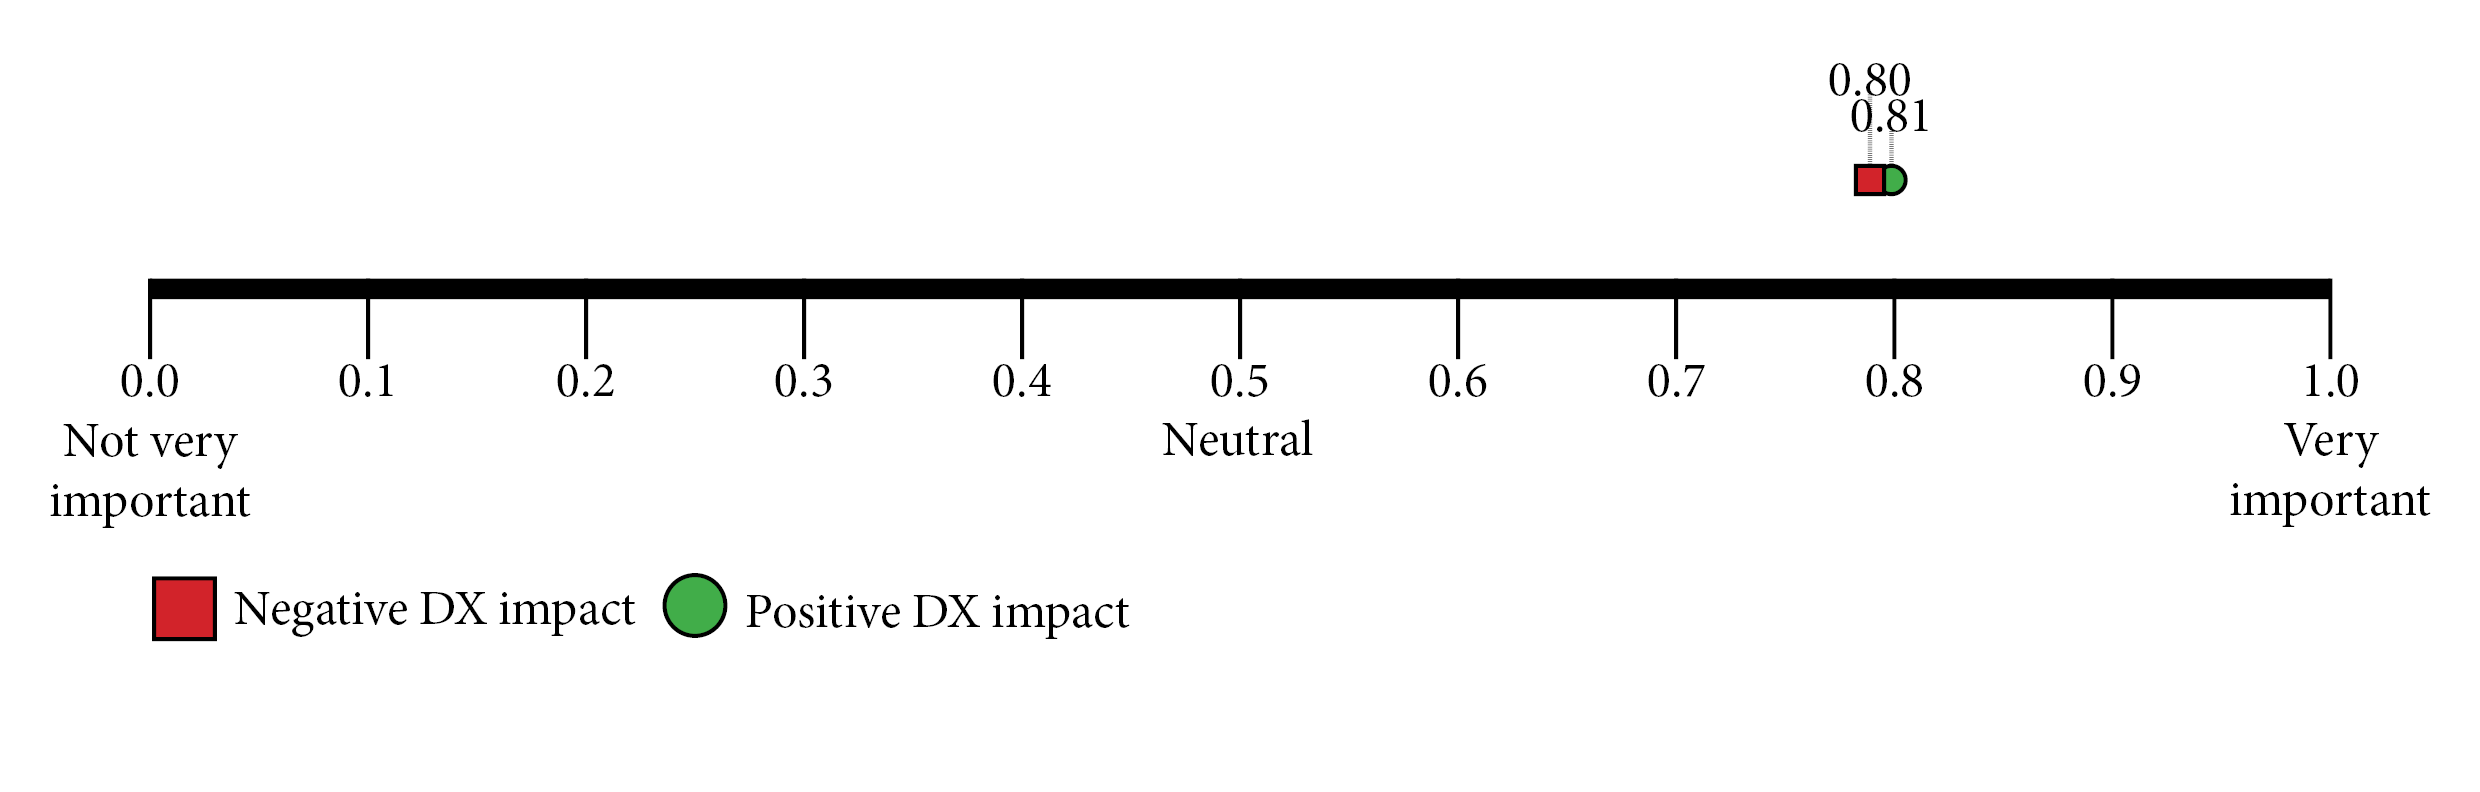
\includegraphics[width=\linewidth]{dxscorelines/dxaspect3.png}
        \caption{Scoring for "The API documentation gives thorough explanations on how it works"}
        \label{fig:aspect3}
    \end{figure}
    Documentation is the heart of a software platform, providing the explanation of how to use it. In figure \ref{fig:aspect3} we can see how it scored. With an average score of 0.82/1.00 it's paramount that this aspect is taken care of. Poor documentation was shown to cause developers to quickly abandon software. It doesn't matter how good your software platform is. If you don't have a good documentation that clearly explains how you're suppose to use it, people will not use your platform. You \textit{must} make sure you explain all parts of your platform. The effort to have thorough documentation is big, but is worth it when you see how important it is. The recommendation is to put a lot of effort into this, listen carefully to any questions you get from users. If a lot of users find the same things difficult, it can be an indicator that the documentation isn't thorough enough. A good method could be to read online discussions, and see what people have difficulty with.\\ \\
    \textbf{Verdict: Very important, always keep in mind. High effort, high payoff.}
    \paragraph{The API has code examples}
    \begin{figure}[H]
        \centering
        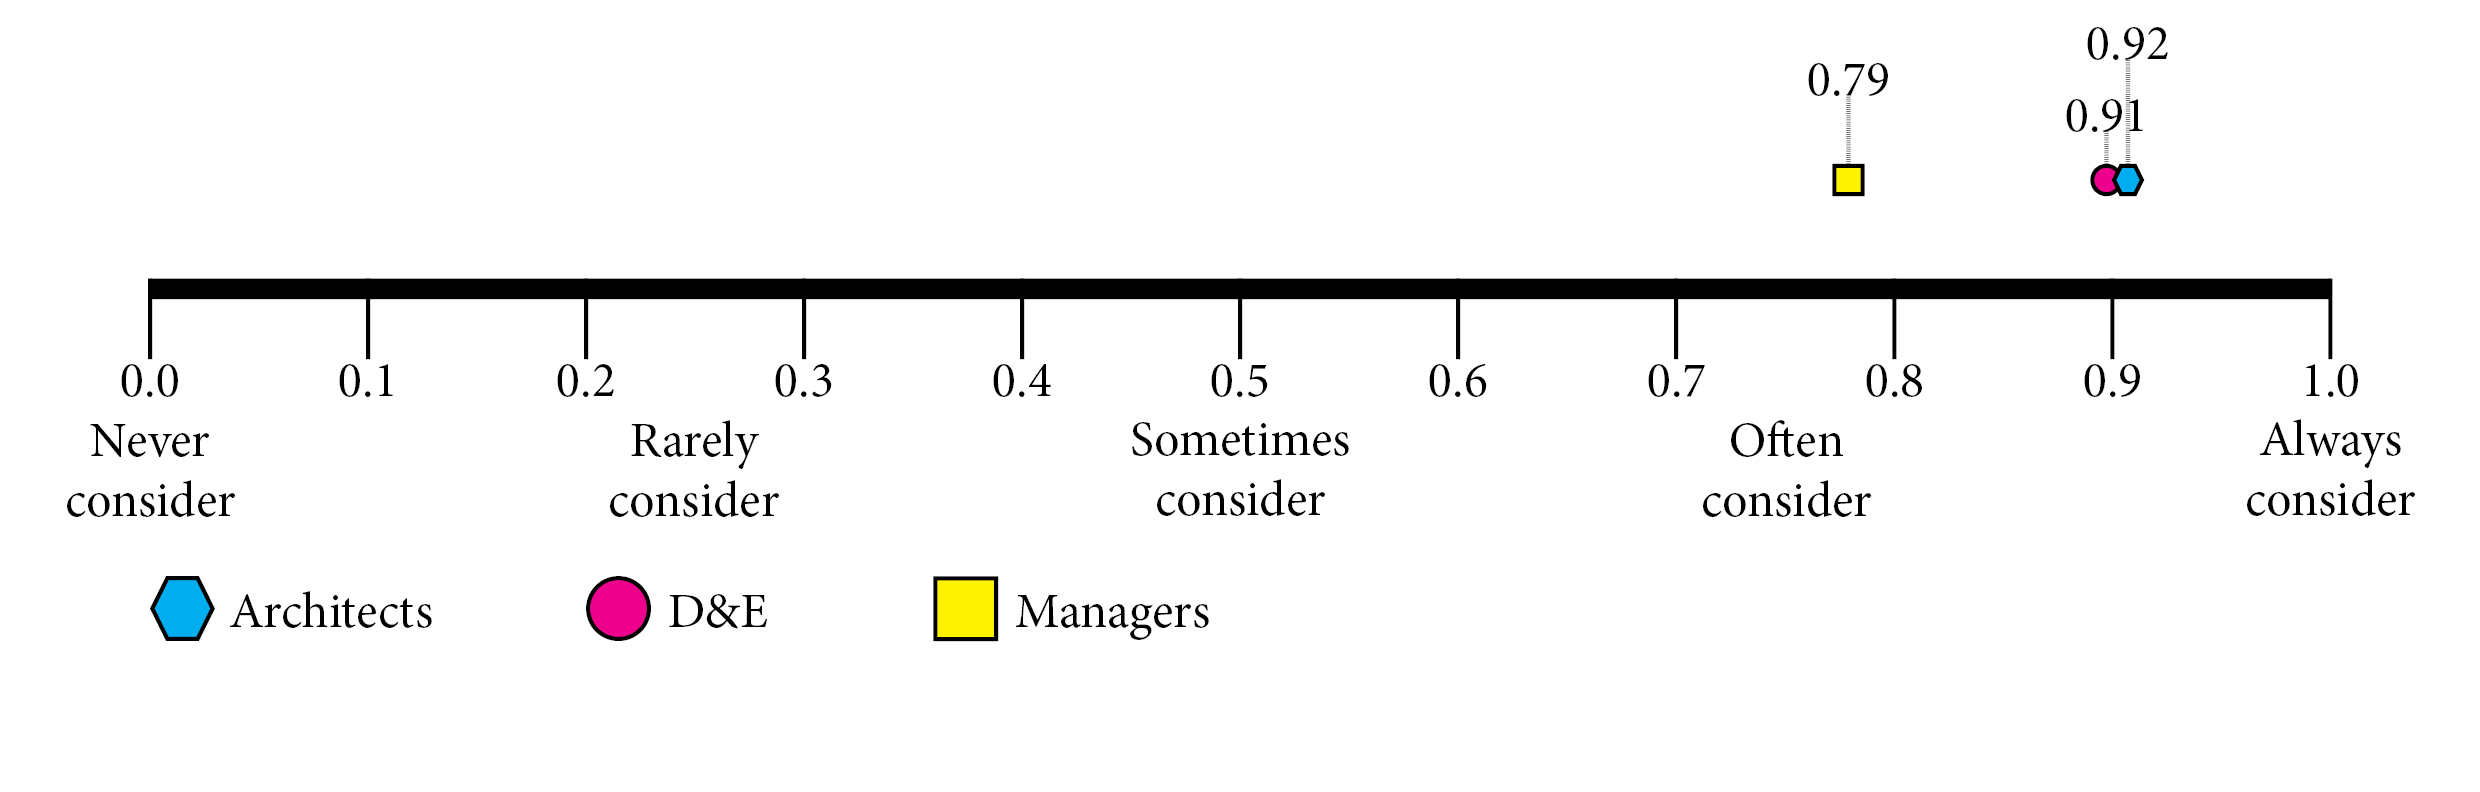
\includegraphics[width=\linewidth]{scorelines/aspect4.png}
        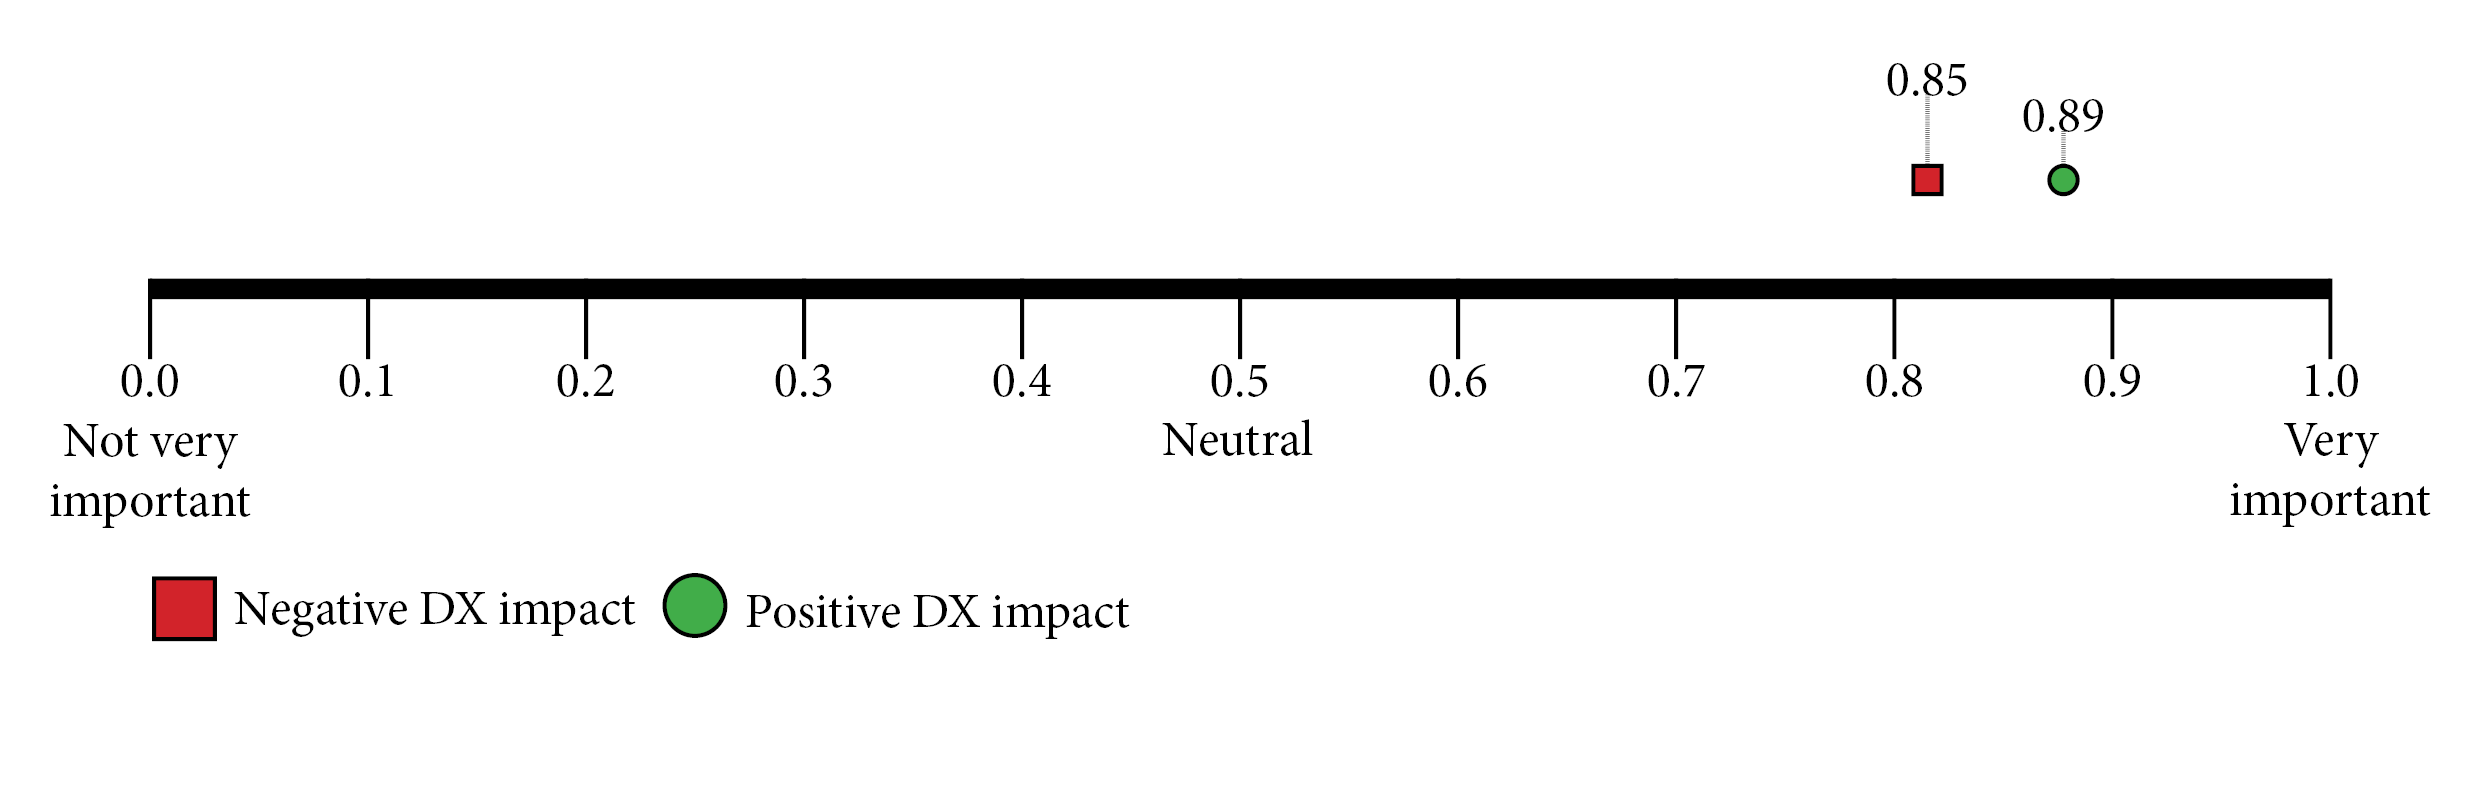
\includegraphics[width=\linewidth]{dxscorelines/dxaspect4.png}
        \caption{Scoring for "The API has code examples"}
        \label{fig:aspect4}
    \end{figure}
    You can explain concepts and methods in text, but often an example is the best way to convey something quickly. The interviews showed that examples is the first thing people look at when encountering documentation. It is therefor important that the example is front and centre in documentation. The examples are used for many things too. It's for copy-pasting into people's projects, getting an overview how things work and are linked together as well as to simply see how things should be used. The effort to construct good examples is quite high. The recommendation is to \texit{always} have a simple example with all methods and concepts, and if possible more advanced examples too. The simple example should be concise, and show the standard situation. It could be tempting to show something fancy. This however increases the risk for confusion. If you're going to show advanced situations, do it in step-by-steps as to not confuse the user. In figure \ref{fig:aspect4} you can see how it scored. With an average score of 0.90/1.00 it's paramount that this aspect is taken care of. It's the first thing users look at, and if they don't understand you risk losing them. \\ \\
    \textbf{Very important, always keep in mind. High effort, high payoff.}
    \paragraph{The documentation doesn’t assume any prior expertise}
    \begin{figure}[H]
        \centering
        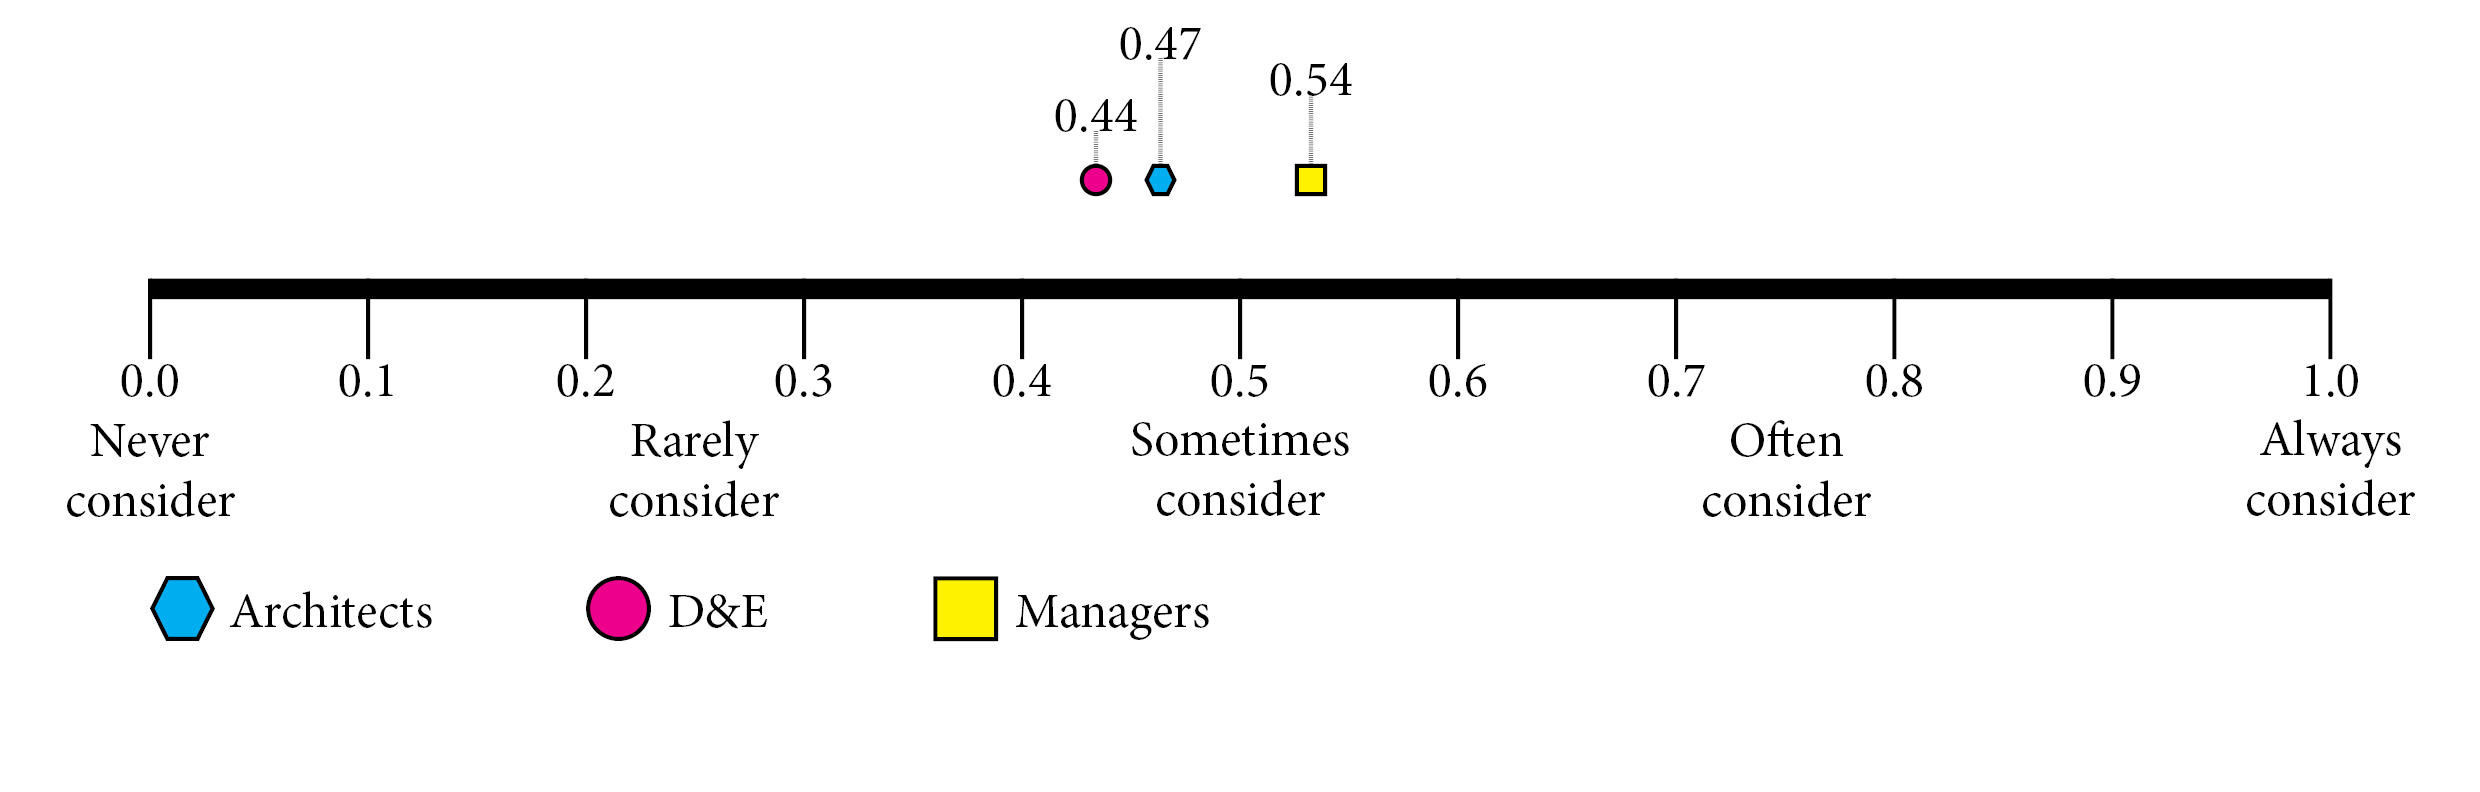
\includegraphics[width=\linewidth]{scorelines/aspect5.png}
        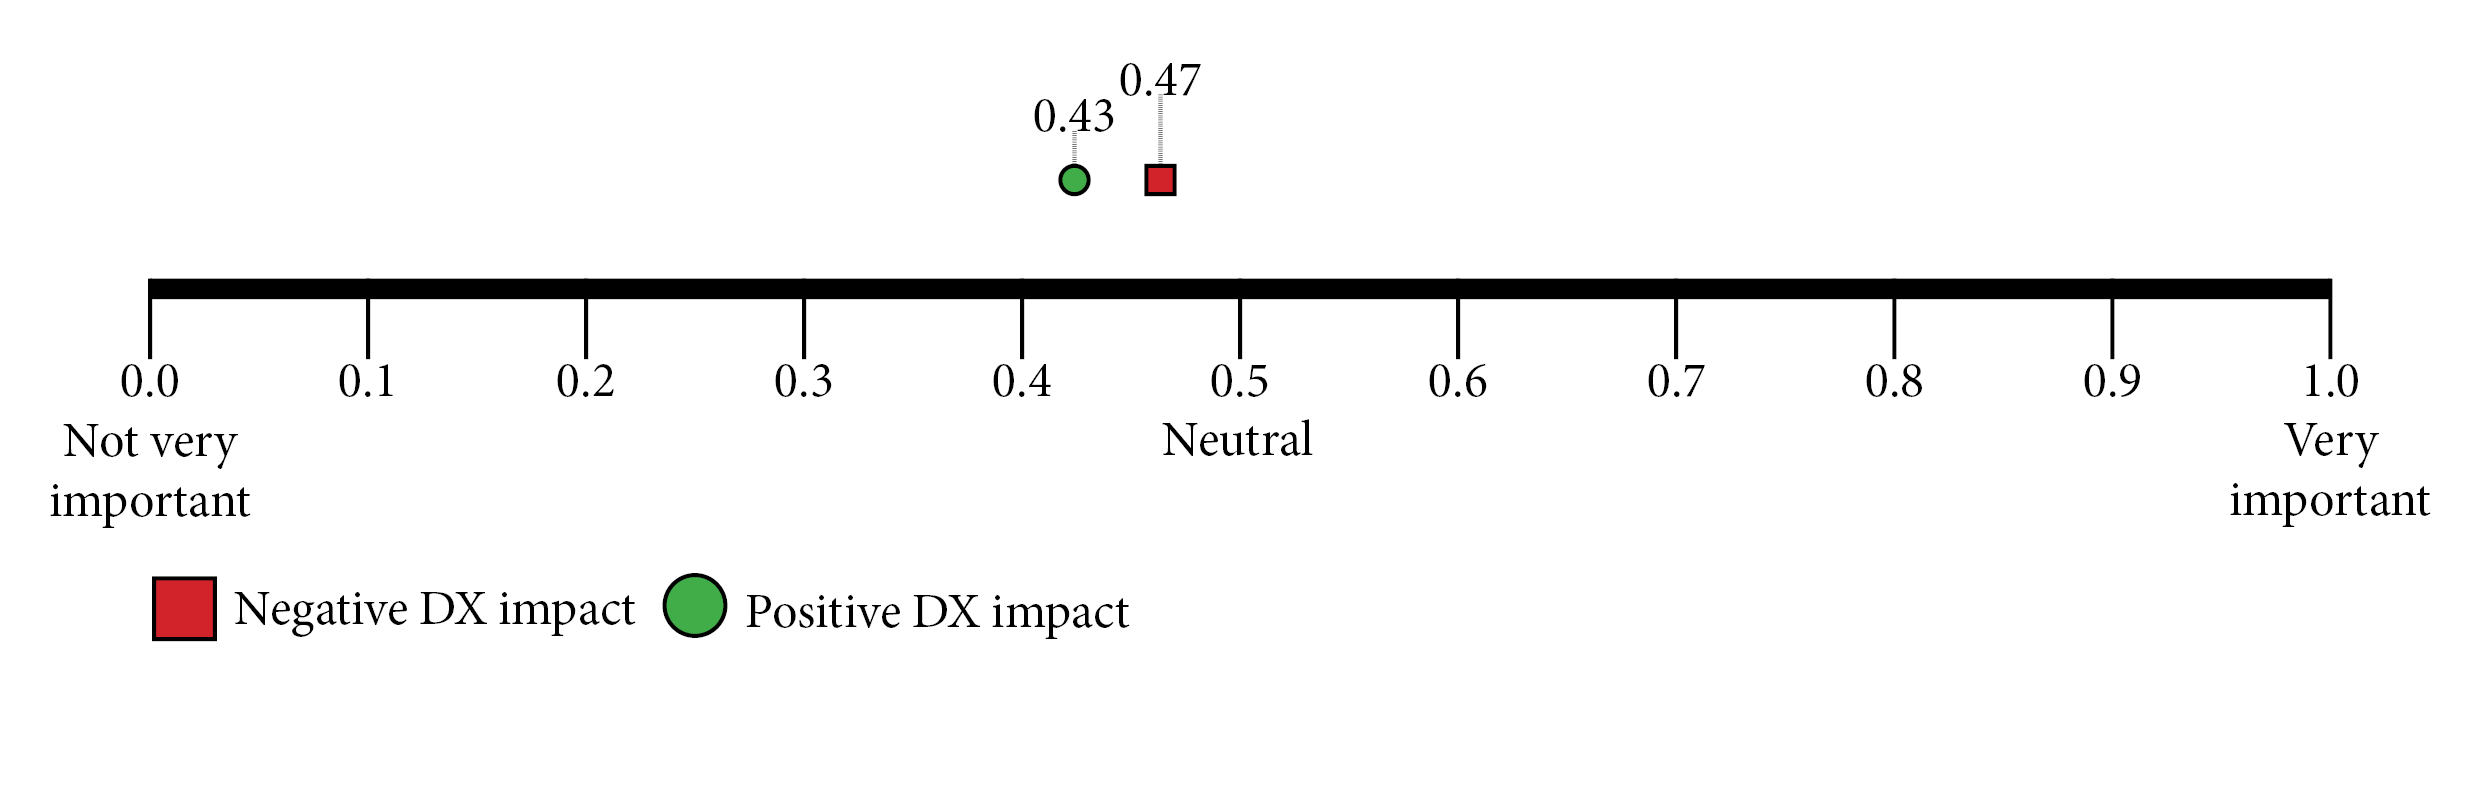
\includegraphics[width=\linewidth]{dxscorelines/dxaspect5.png}
        \caption{Scoring for "The documentation doesn’t assume any prior expertise"}
        \label{fig:aspect5}
    \end{figure}
    Software platforms will naturally have concepts that are new to people. Whenever a new concept is used, you risk confusing the user if it's not explained. In figure \ref{fig:aspect5} you can see that it does not score very high, with an average of 0.47/1.00. This doesn't mean that it can be completely ignored, but people are not scared away by new concepts. The recommendation is to link to an explanations of new concepts where ever they're used. This effort is not very big, but solves the problem. \\ \\
    \textbf{Verdict: Not very important, but don't ignore. Low effort, medium payoff.}
    \paragraph{The documentation has consistent language}
    \begin{figure}[H]
        \centering
        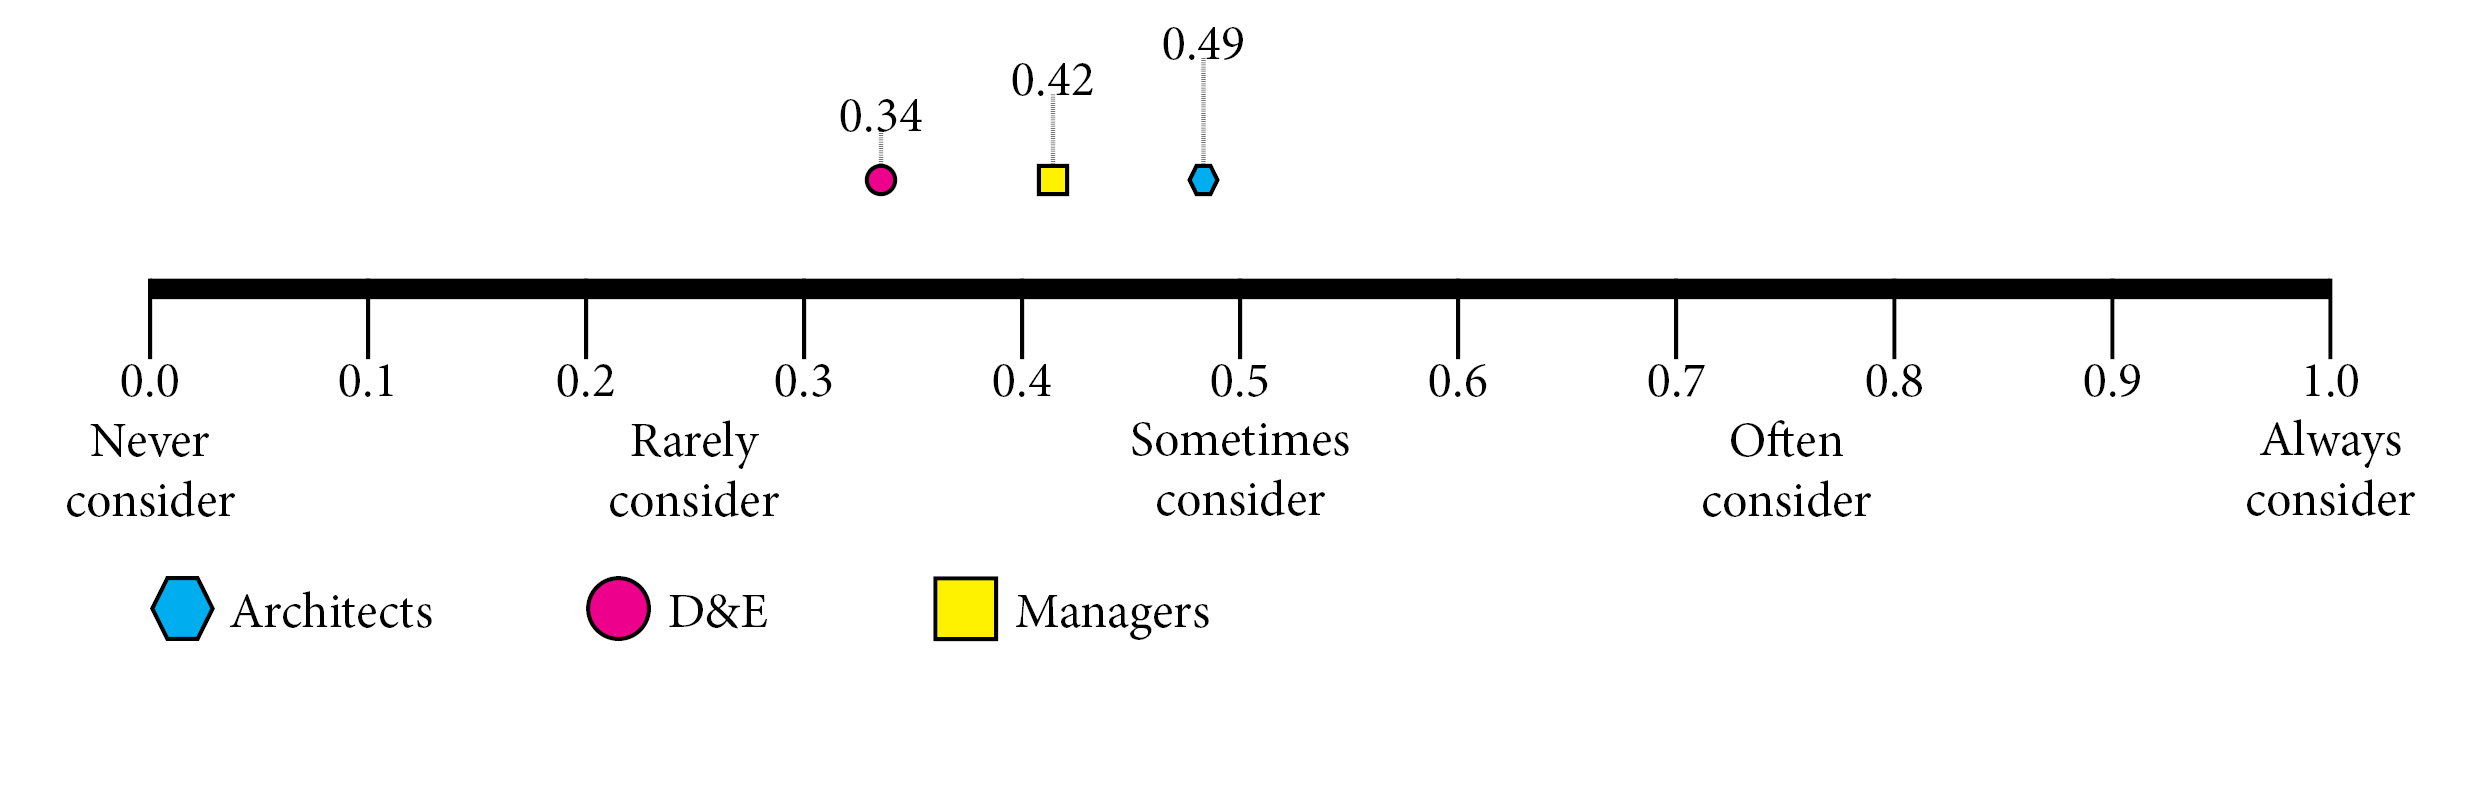
\includegraphics[width=\linewidth]{scorelines/aspect6.png}
        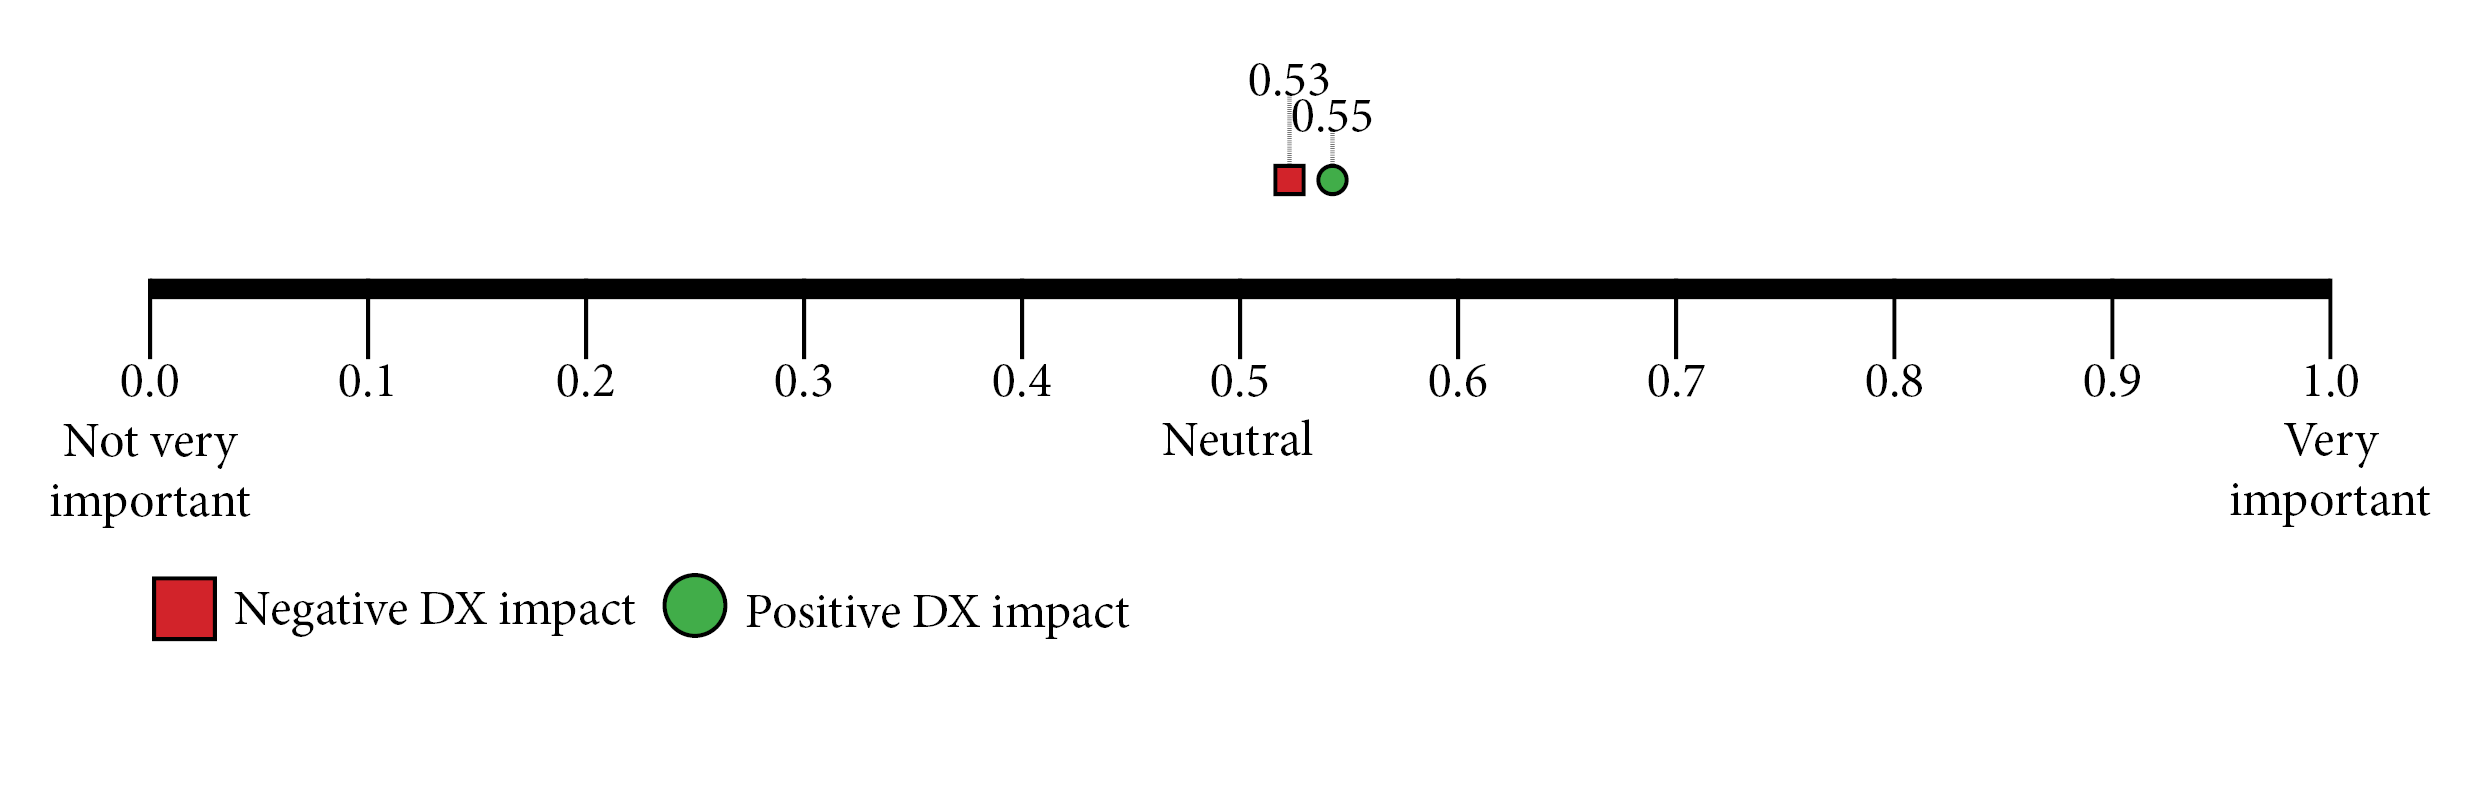
\includegraphics[width=\linewidth]{dxscorelines/dxaspect6.png}
        \caption{Scoring for "The documentation has consistent language"}
        \label{fig:aspect6}
    \end{figure}
    Having consistent language is an indicator of a documentation that has been thoroughly reviewed and worked with. In figure \ref{fig:aspect6} however we can see that it scores quite low, with an average of 0.41/1.00. A documentation with inconsistency language is still very much usable, it just increases the risk for confusion. The effort to fix an already inconsistent documentation is very high. The recommendation is to define a vocabulary that should be used by the documentation writers before starting to write documentation, or from now on if the documentation has already been written. This will ensure that new documentation has consistency, as long as the documentation make sure to use the vocabulary. Because of the high effort, and low importance according to this research, going through documentation and fixing inconsistency should not be of very high priority.\\ \\
    \textbf{Verdict: Not very important, but don't ignore. High effort, low payoff.}
    \paragraph{The documentation is easy to navigate}
    \begin{figure}[H]
        \centering
        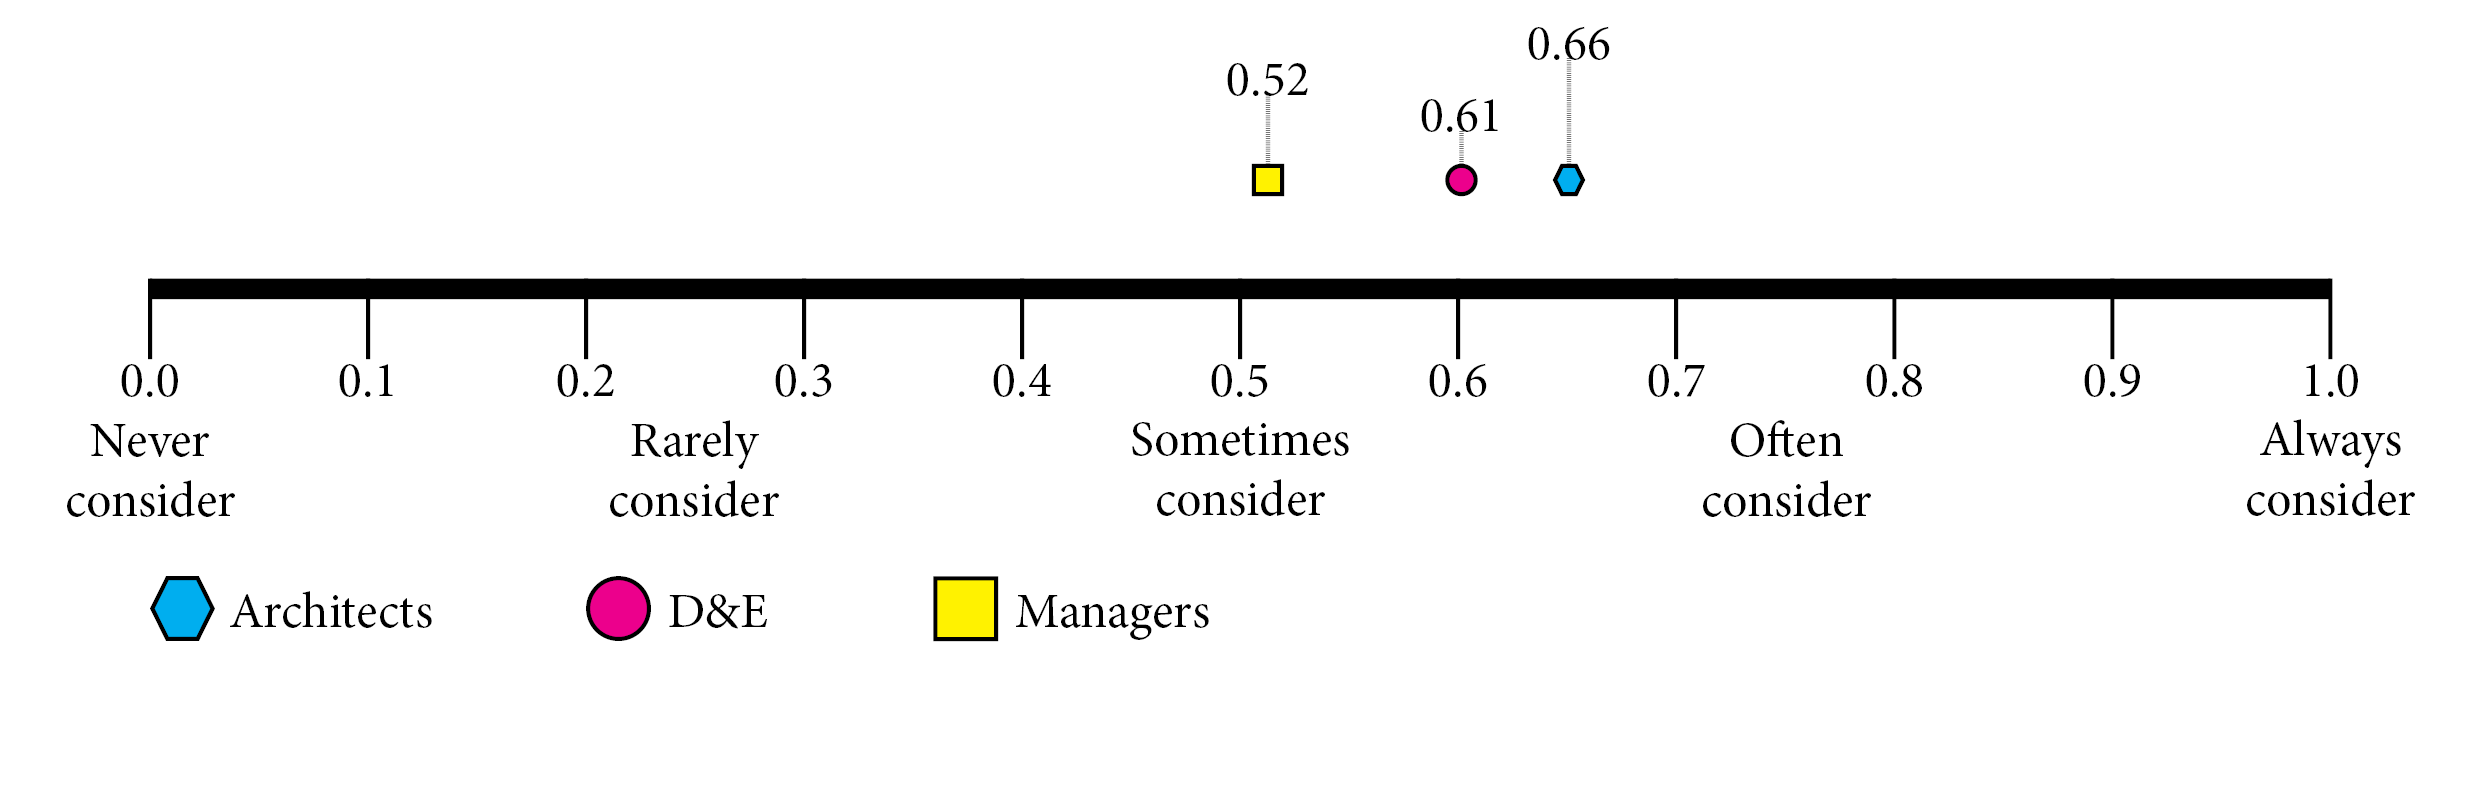
\includegraphics[width=\linewidth]{scorelines/aspect7.png}
        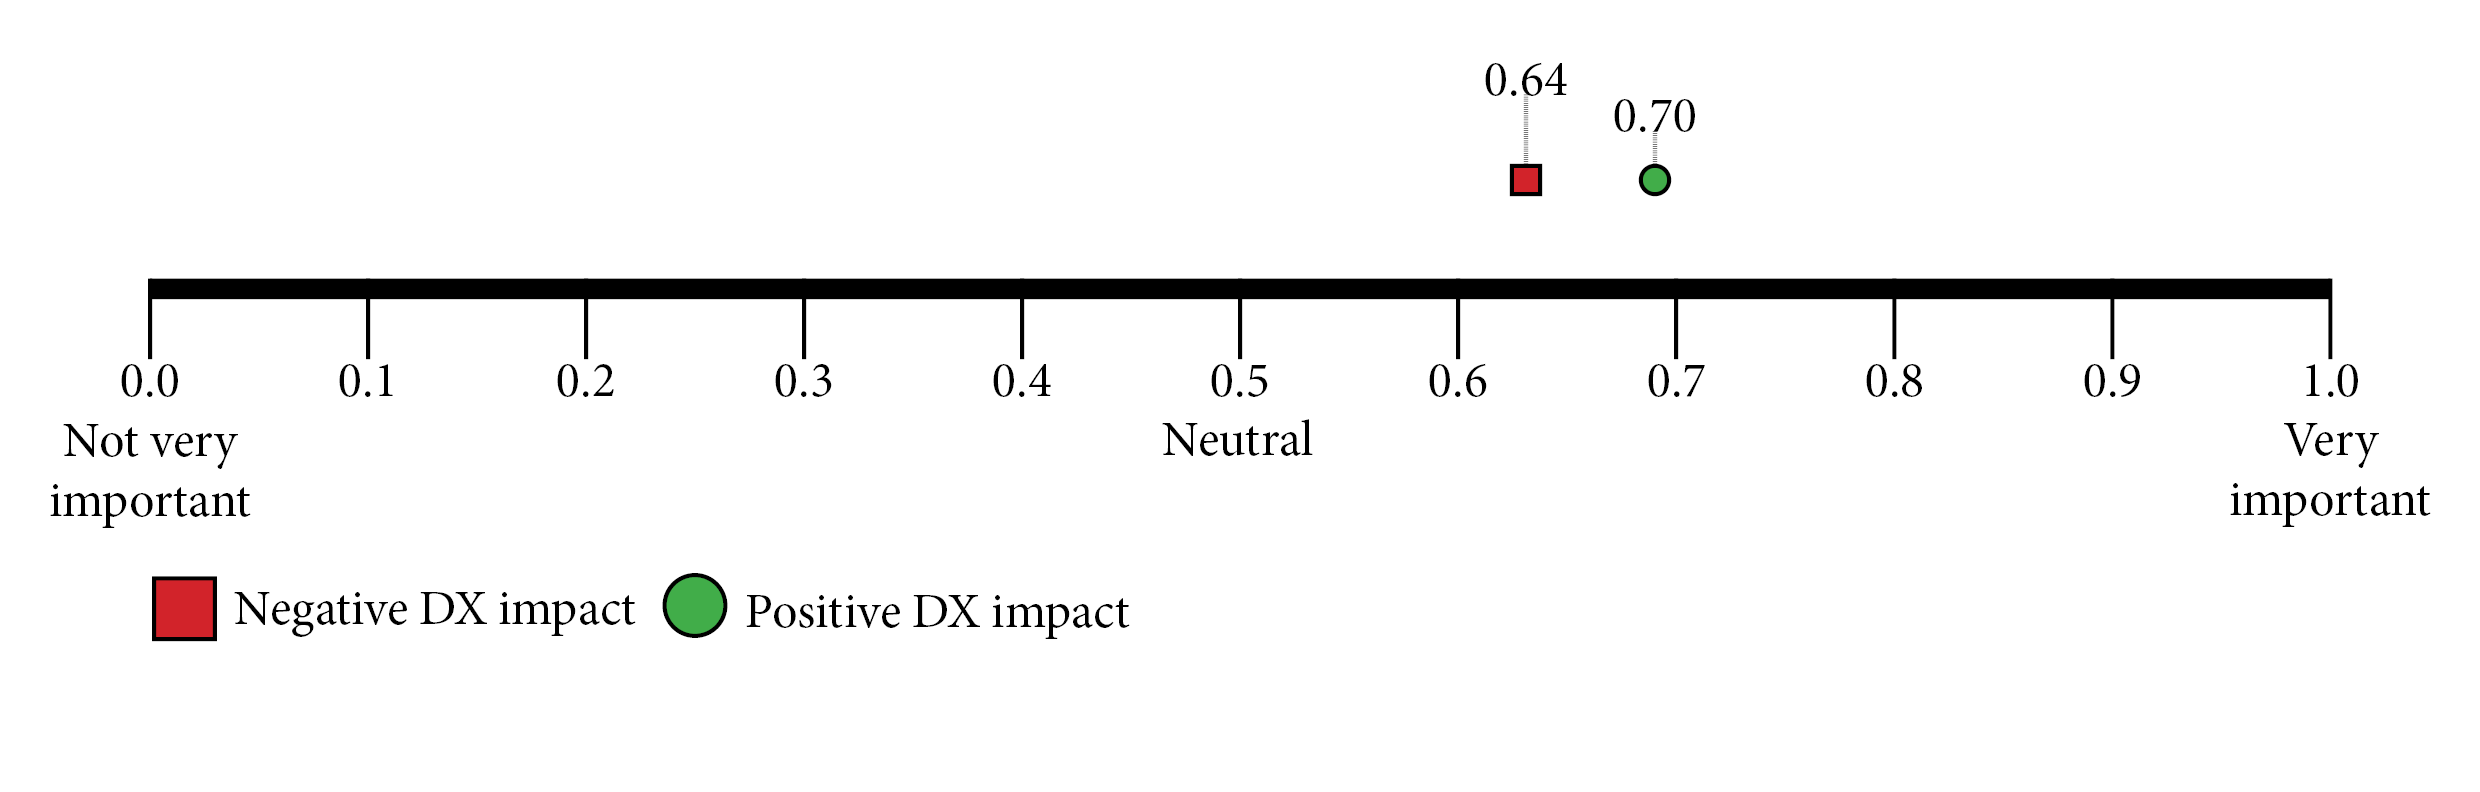
\includegraphics[width=\linewidth]{dxscorelines/dxaspect7.png}
        \caption{Scoring for "The documentation is easy to navigate"}
        \label{fig:aspect7}
    \end{figure}
    As mentioned before, developers are impatient people. A documentation that is easy to navigate, means developers can find what they're looking for quicker. The recommendation is therefor to have a clear navigation structure, with carefully chosen titles that makes the user understand what each link will lead them to. For larger pages, having a table of contents at the top that shows what sections it contains is also recommended. For smaller sub-pages a short paragraph could be good to explain to the user what he or she can expect to find on the page. This gives the possibility to the user to be more efficient when searching for specific things. The effort to do this can be somewhat high, especially the careful title naming. The titles can easily be too vague or ambivalent. Having an efficient search function for your documentation will also make the navigation more easy. To implement this is a higher effort than structuring the documentation. We therefor recommend to start with the structure, and after that work on the search function. \\ \\
    \textbf{Verdict: Somewhat important, keep in mind. Medium-high effort, medium payoff.}
    
    \paragraph{The official website looks professional}
    \begin{figure}[H]
        \centering
        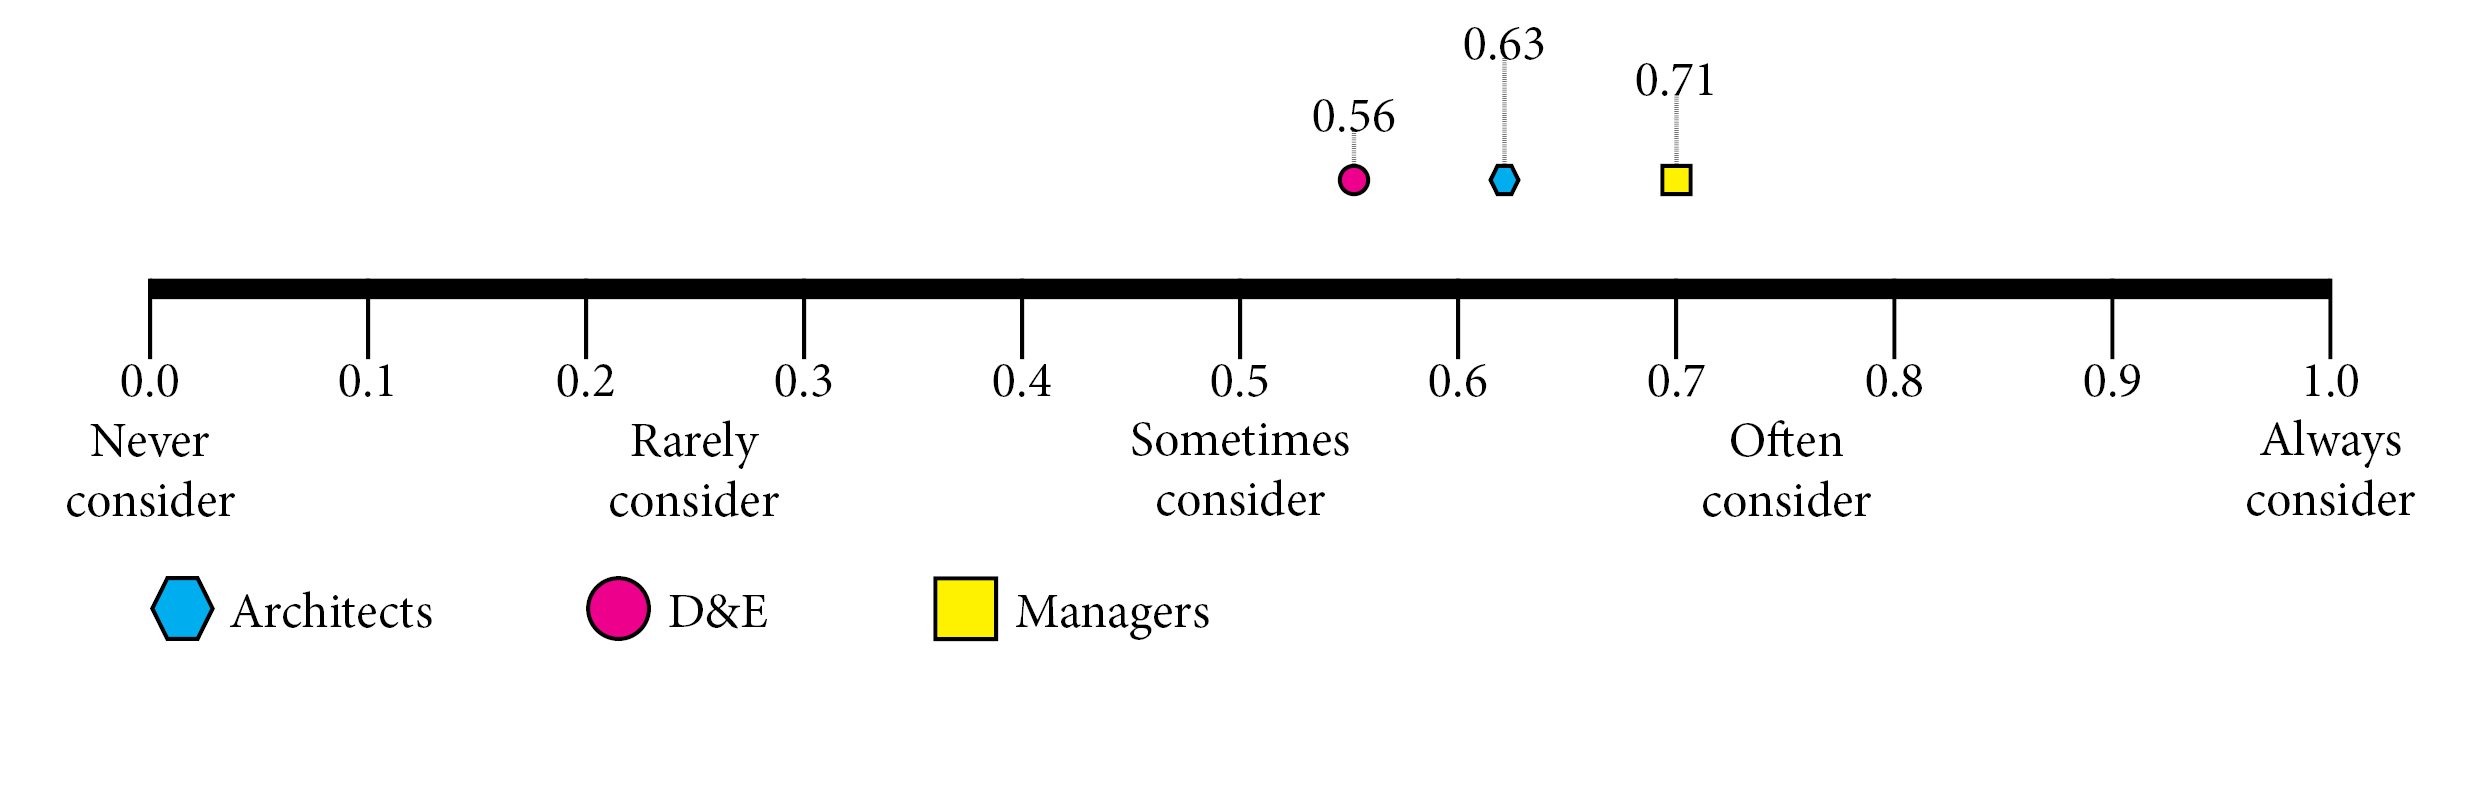
\includegraphics[width=\linewidth]{scorelines/aspect8.png}
        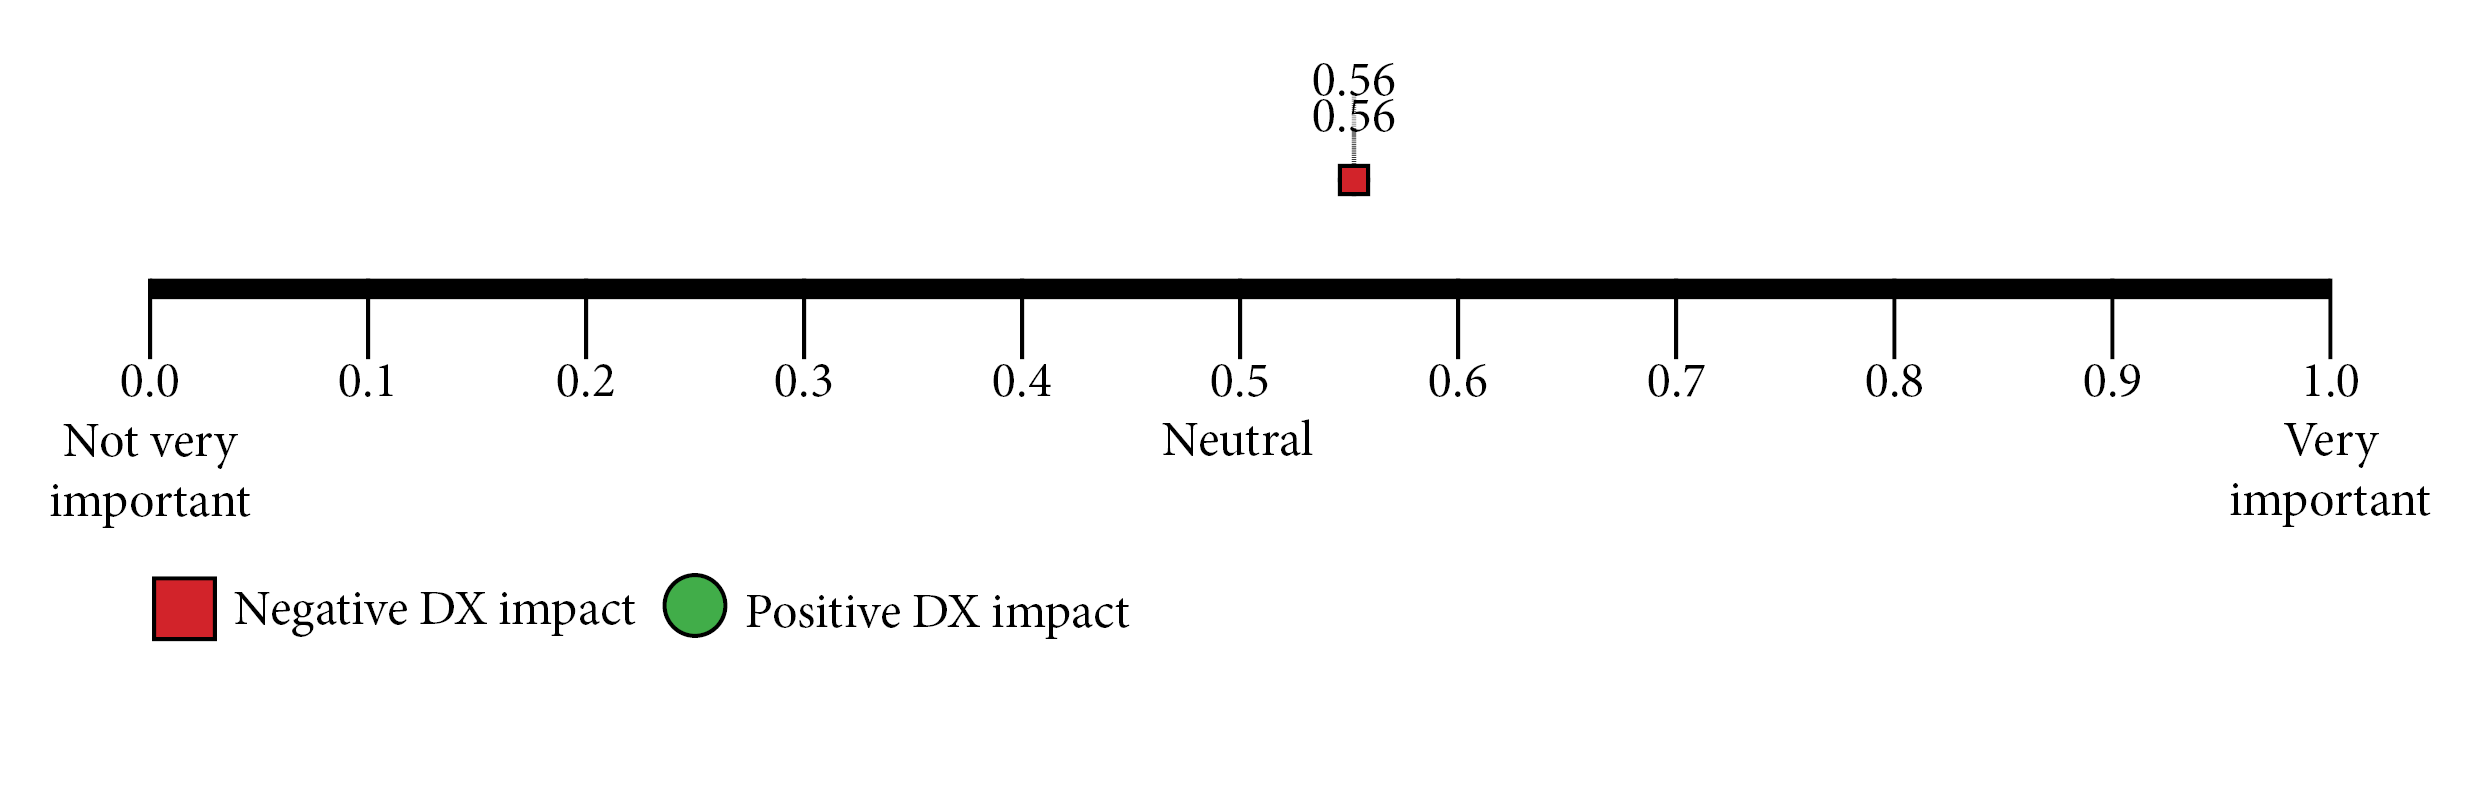
\includegraphics[width=\linewidth]{dxscorelines/dxaspect8.png}
        \caption{Scoring for "The official website looks professional"}
        \label{fig:aspect8}
    \end{figure}
    The official website is often a company's face outwards, and a user's first encounter with the company. You should not downplay the importance of first impressions. In figure \ref{fig:aspect8} we can see that it scored somewhere in between 'Sometimes consider' and 'Often consider' with the average score of 0.60/1.00. The recommendation is therefor to spend some time to make sure your official website looks professional. Test it for different browsers and devices. The effort to do this should not be high for a software company who creates software platforms. If a company whom provides software platform solutions cannot provide a professional looking website, the impression it gives is that they won't provide a good platform either. As seen in figure \ref{fig:aspect8} it's more important to managers. If you cater to these, this aspect is even more important. 
    \\ \\
    \textbf{Verdict: Somewhat important, keep in mind. Medium effort, medium payoff.}
    
    \paragraph{The pricing of the software}
    \begin{figure}[H]
        \centering
        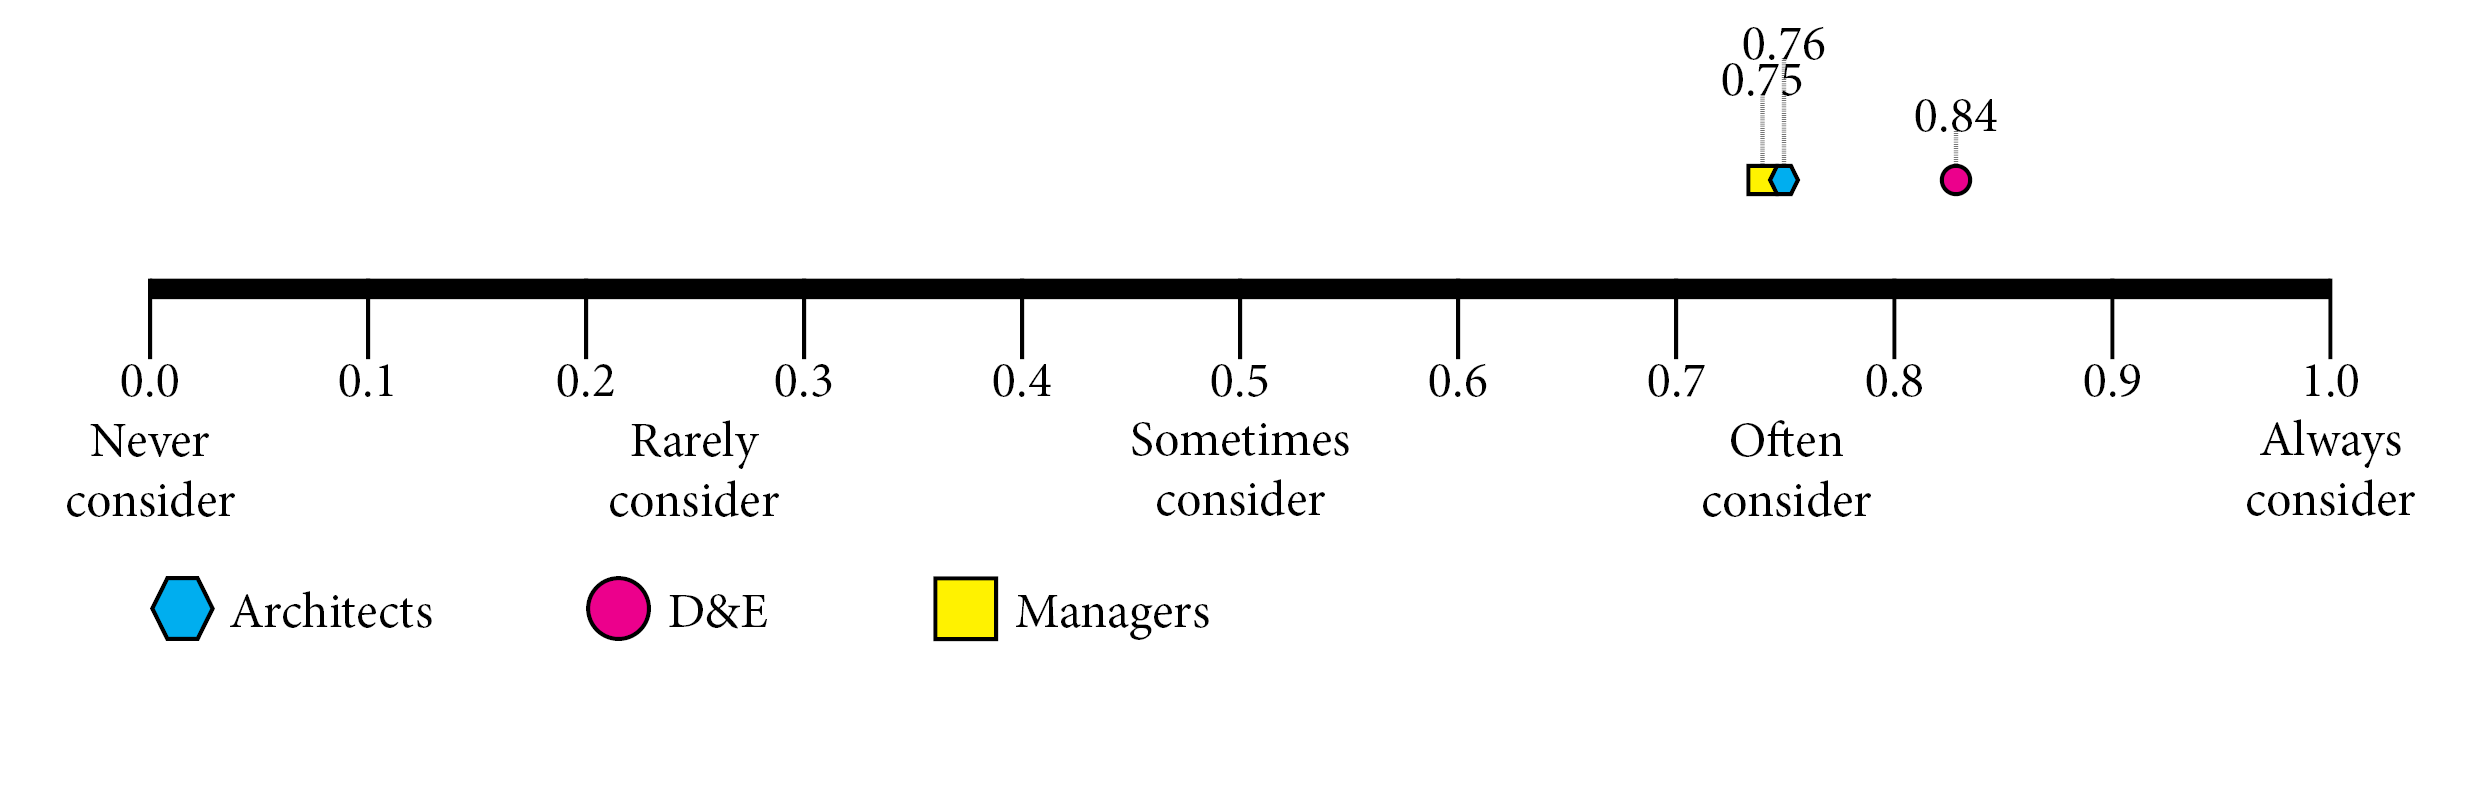
\includegraphics[width=\linewidth]{scorelines/aspect9.png}
        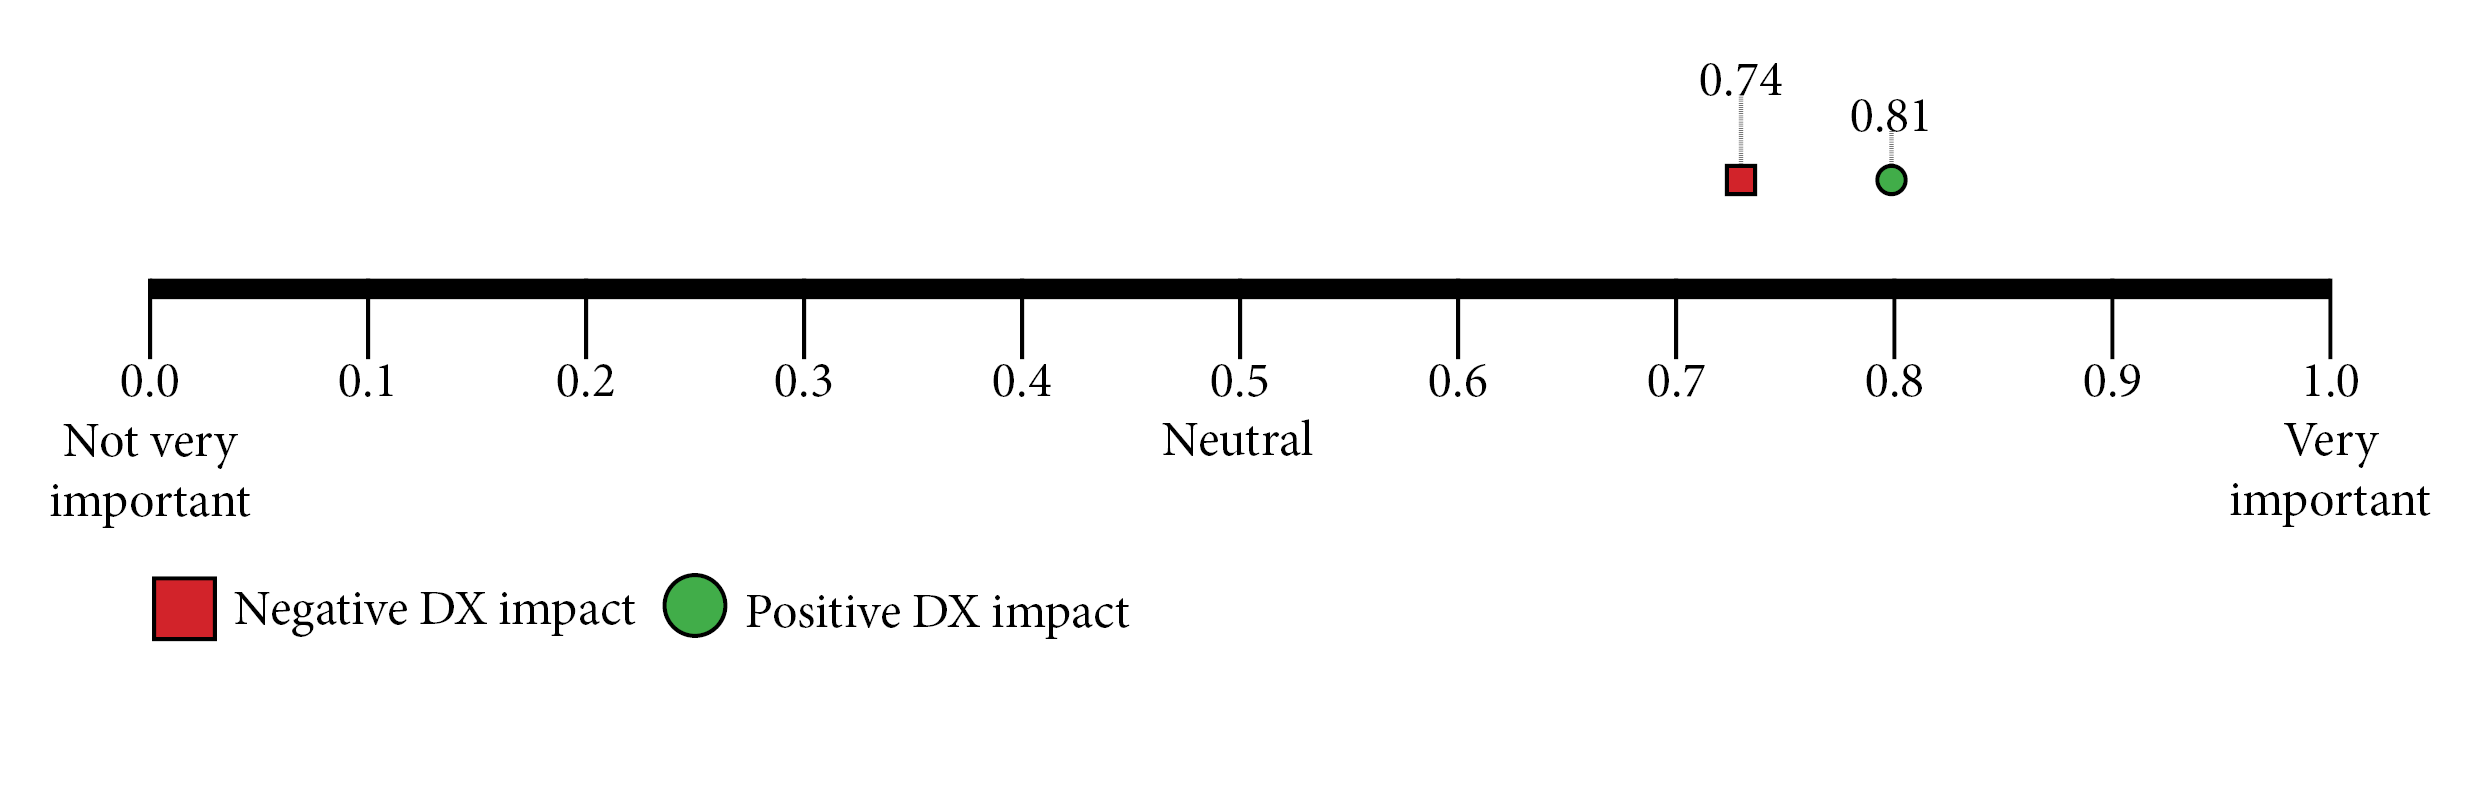
\includegraphics[width=\linewidth]{dxscorelines/dxaspect9.png}
        \caption{Scoring for "The pricing of the software"}
        \label{fig:aspect9}
    \end{figure}
    Money always plays a roll in any company, and the price of a software cannot be ignored. You can make money from your software in many ways, through licensing, subscriptions, support contract, and more. It's out of the scope of this research paper on how one should make money from software platforms. The recommendation for pricing, in order to give a good experience for developers, is to clearly state the pricing of the software platform. Whichever money making model the software platform uses, the cost to inquire it for a developer should not be hidden away. \\ \\
    \textbf{Verdict: Important, keep in mind. Low effort, high payoff.}
    
    \paragraph{The release- and change notes are thorough}
    \begin{figure}[H]
        \centering
        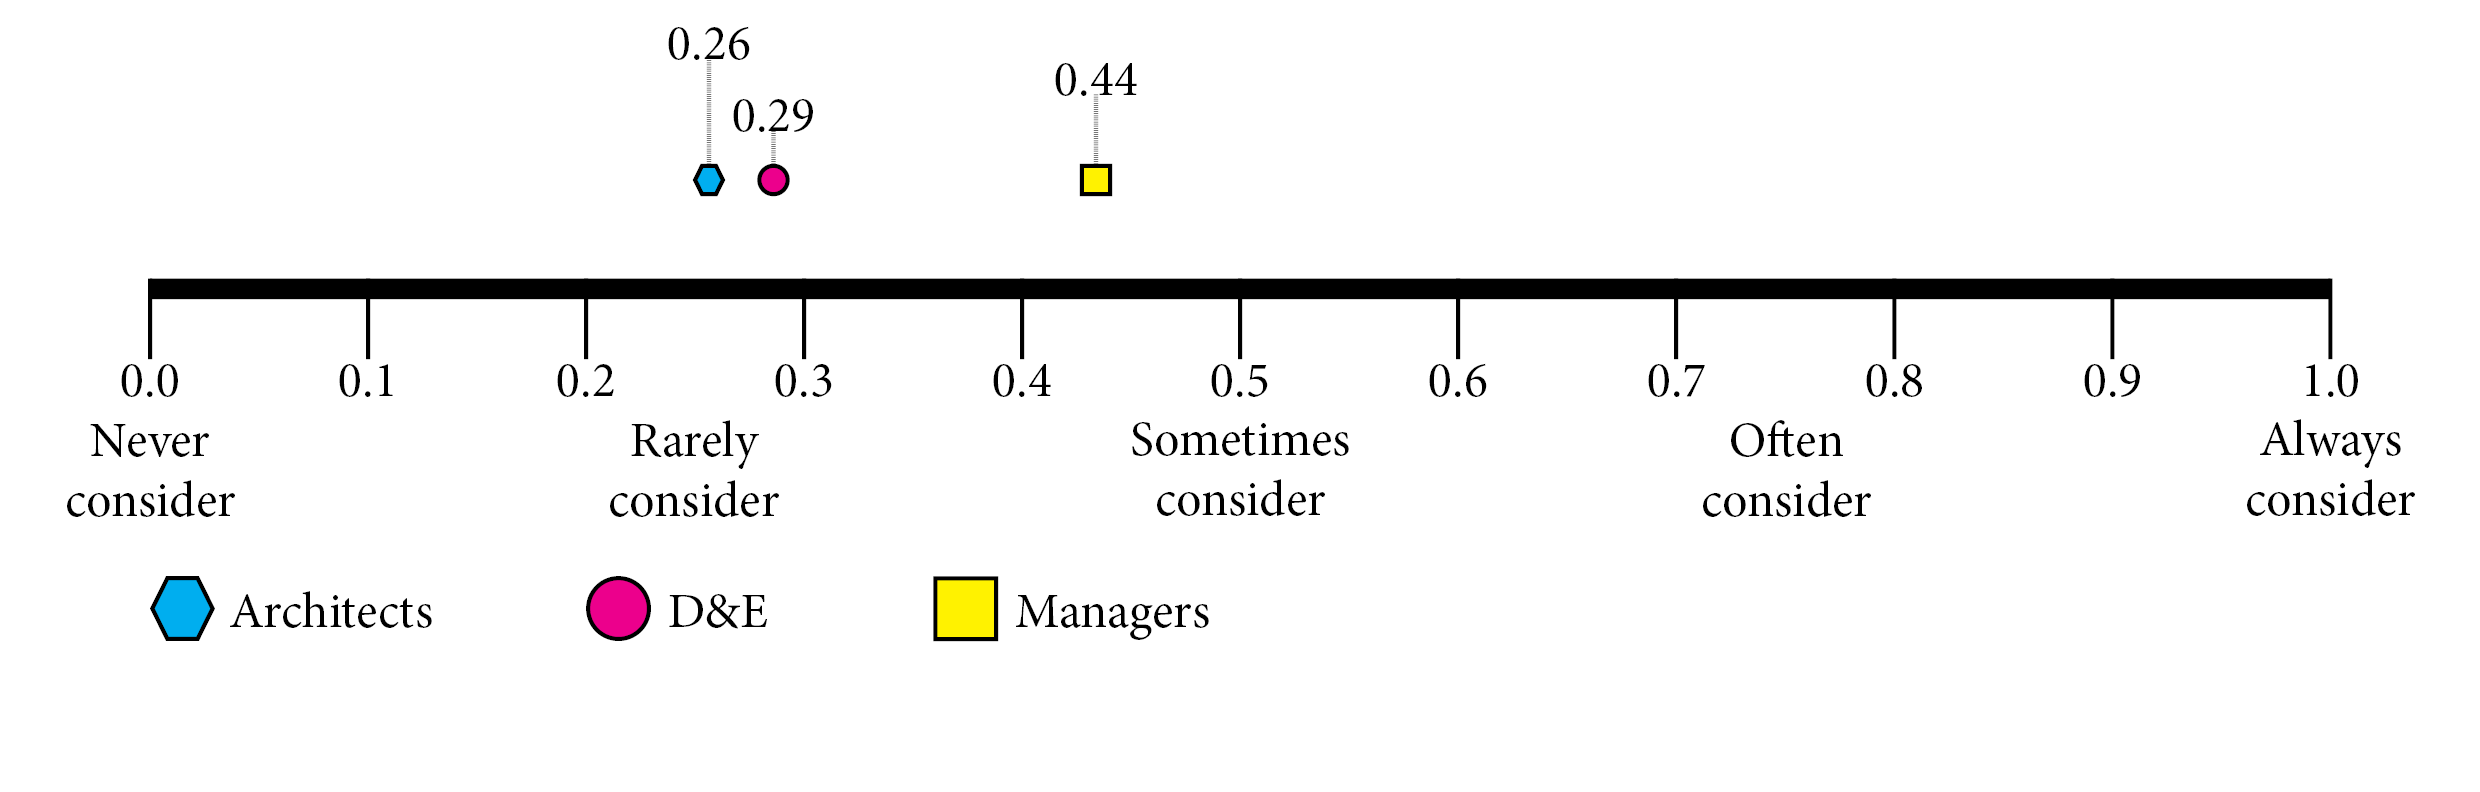
\includegraphics[width=\linewidth]{scorelines/aspect10.png}
        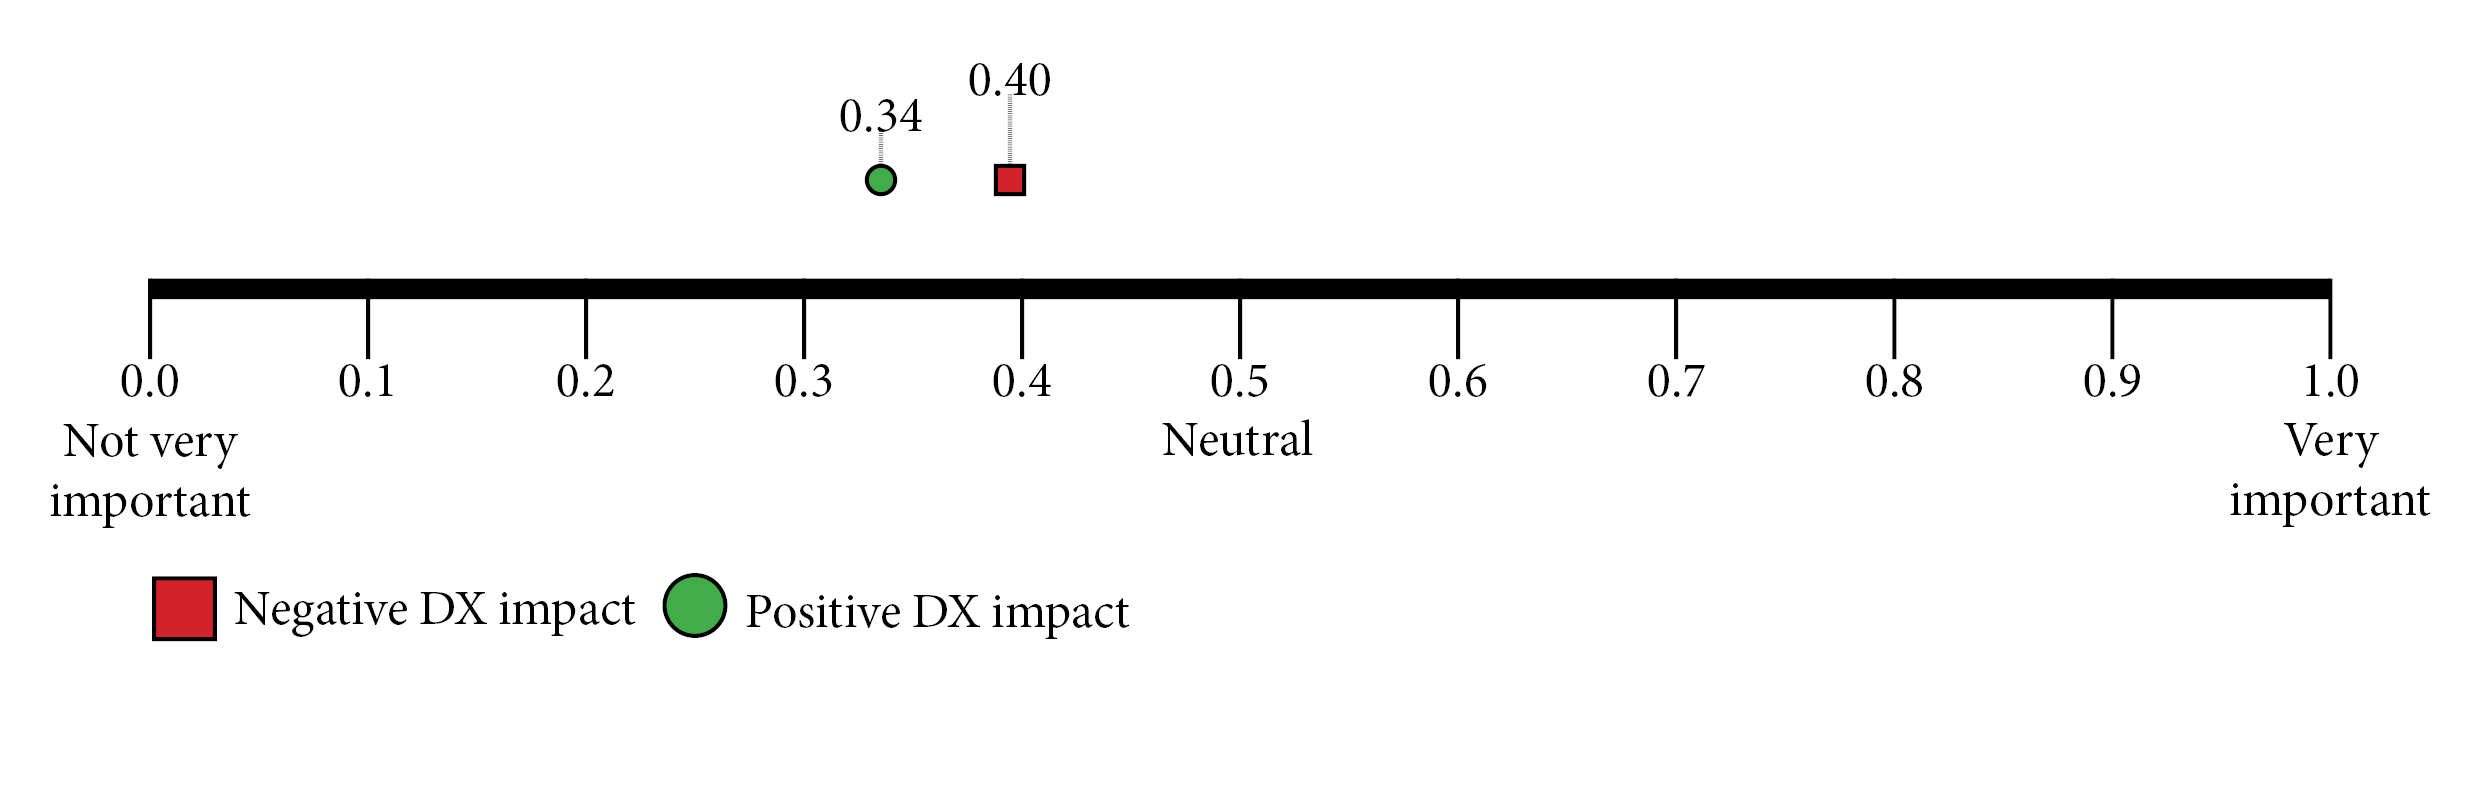
\includegraphics[width=\linewidth]{dxscorelines/dxaspect10.png}
        \caption{Scoring for "The release- and change notes are thorough"}
        \label{fig:aspect10}
    \end{figure}
    Release notes was shown to be a quite non-important aspect, as seen in figure \ref{fig:aspect10}, especially for the people who are supposedly using them: developers and architects. The interviews showed that release notes are a last resort for people, and ignored as much as possible. There recommendation is therefor to not spend too much time on release notes. But make sure to not ignore them. If you make sure to have good commit messages, these can act as a good base for writing the release notes. This minimises the time that has to be spent on writing the release notes.\\ \\
    \textbf{Verdict: Not important, but don't ignore. Medium effort, low payoff.}
    
    \paragraph{The software has the same features on all different platforms}
    \begin{figure}[H]
        \centering
        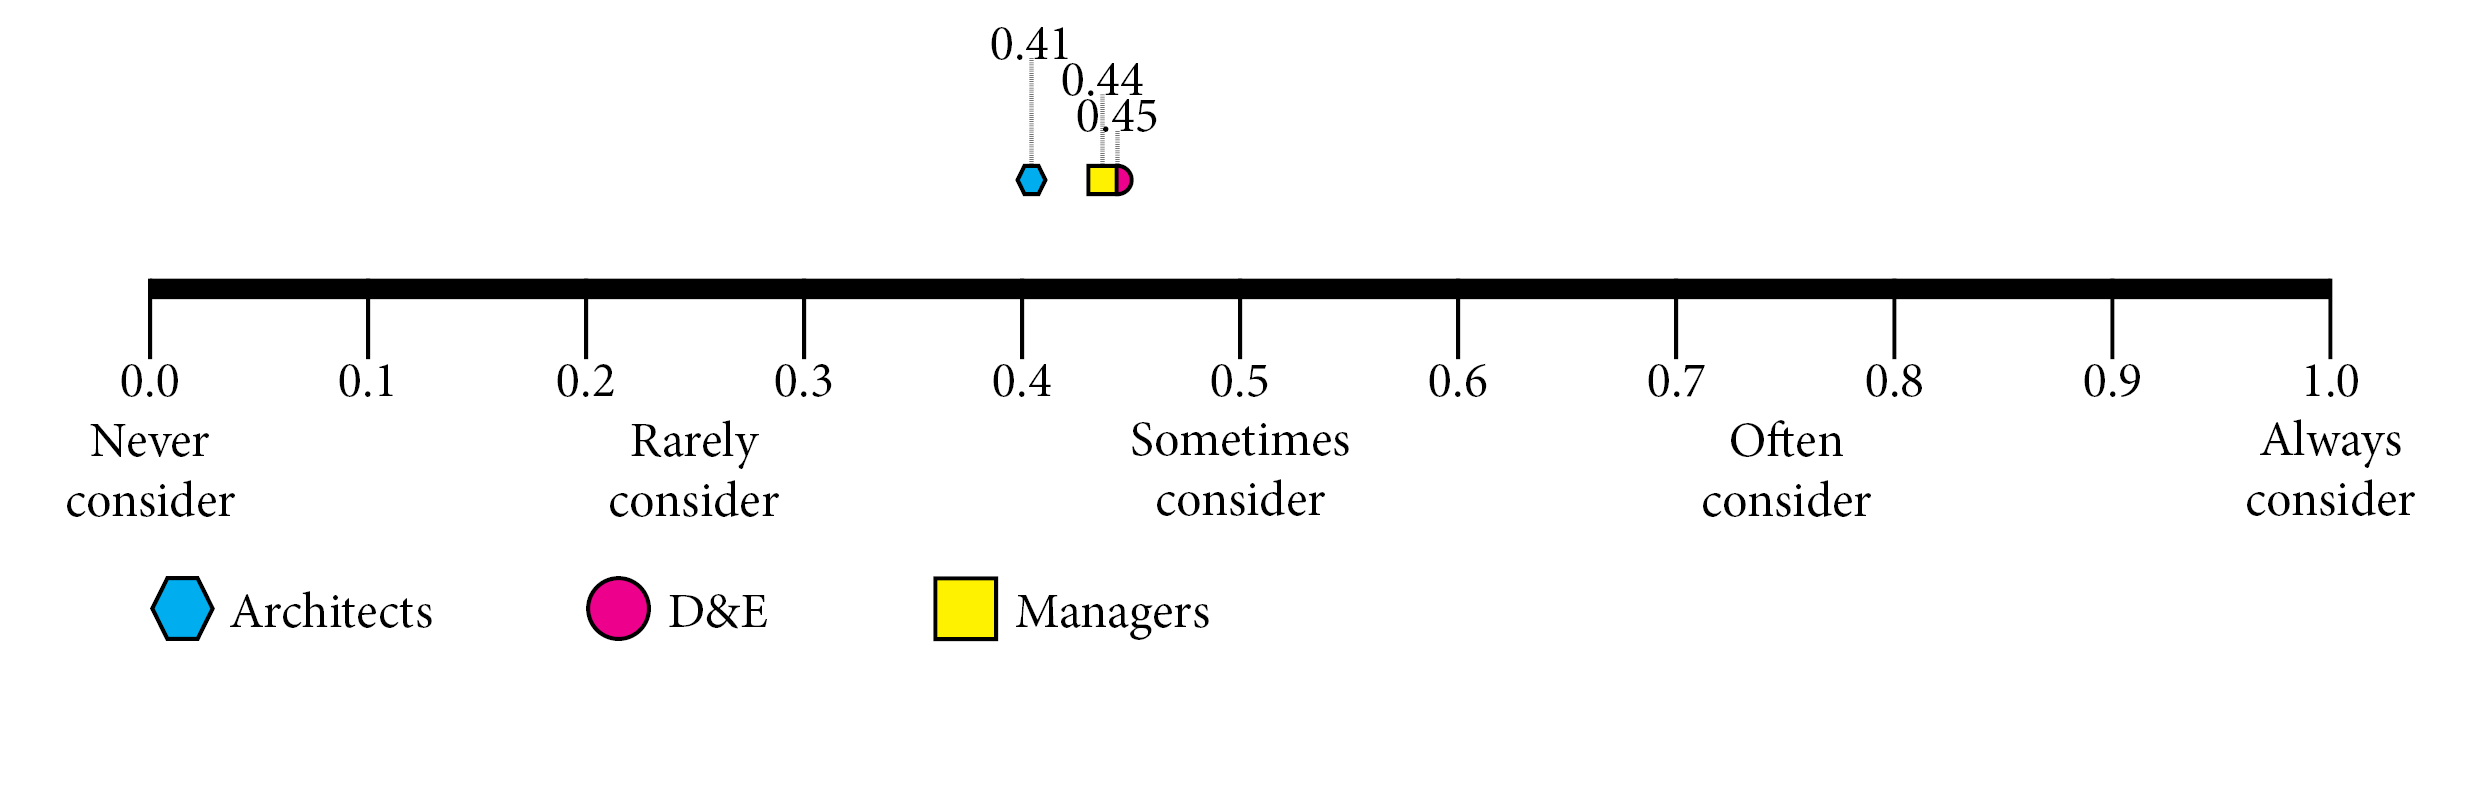
\includegraphics[width=\linewidth]{scorelines/aspect11.png}
        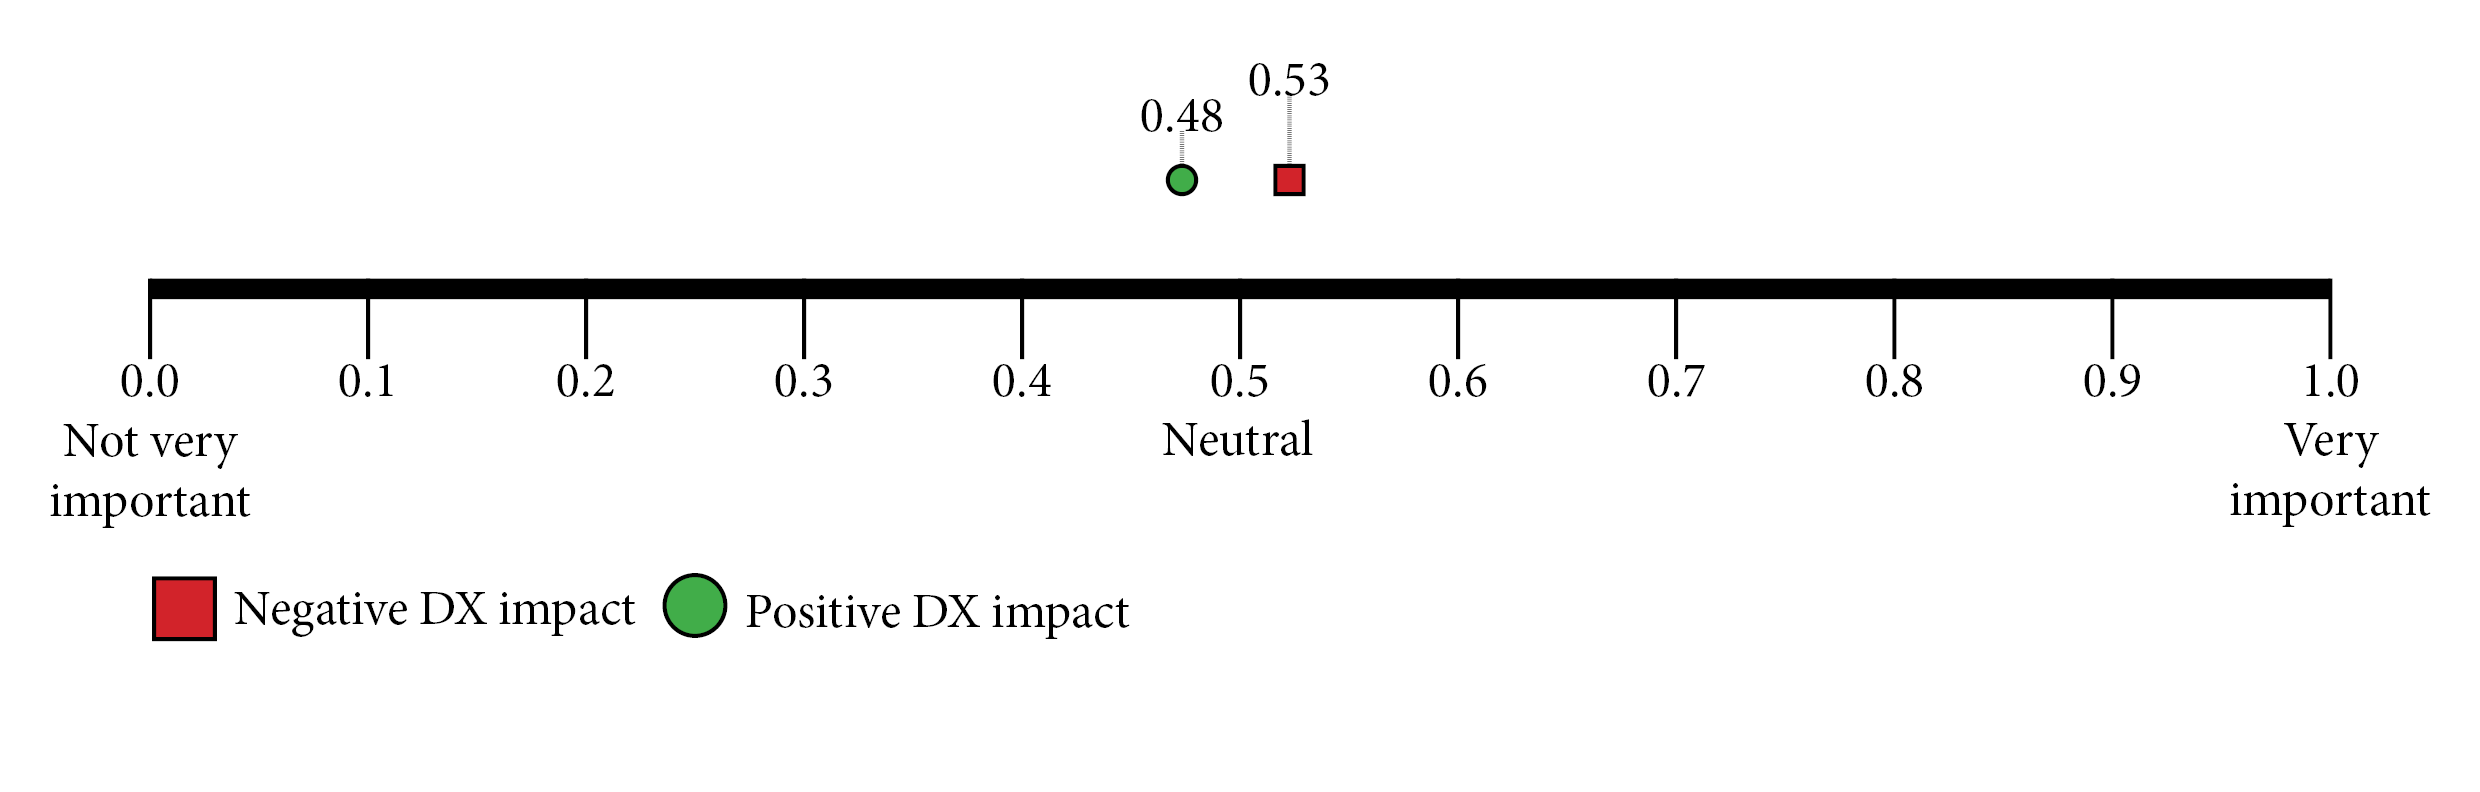
\includegraphics[width=\linewidth]{dxscorelines/dxaspect11.png}
        \caption{Scoring for "The software has the same features on all different platforms"}
        \label{fig:aspect11}
    \end{figure}
    If your software platform supports many different platforms, such as operation systems and browsers, it's takes time and effort to make sure that they work the same in all situations. In figure \ref{fig:aspect11} we see that this scores kind of low. The effort however to make sure that all features exist on all platforms is very high. The recommendation is therefor to clearly state to the users what features are offered on what platforms. But be aware that the effort to keep the features consistent on all platforms may not have a big payoff. \\ \\
    \textbf{Verdict: Not very important. High effort, low-medium payoff.}
    
    \paragraph{The software is compatible with different platforms}
    \begin{figure}[H]
        \centering
        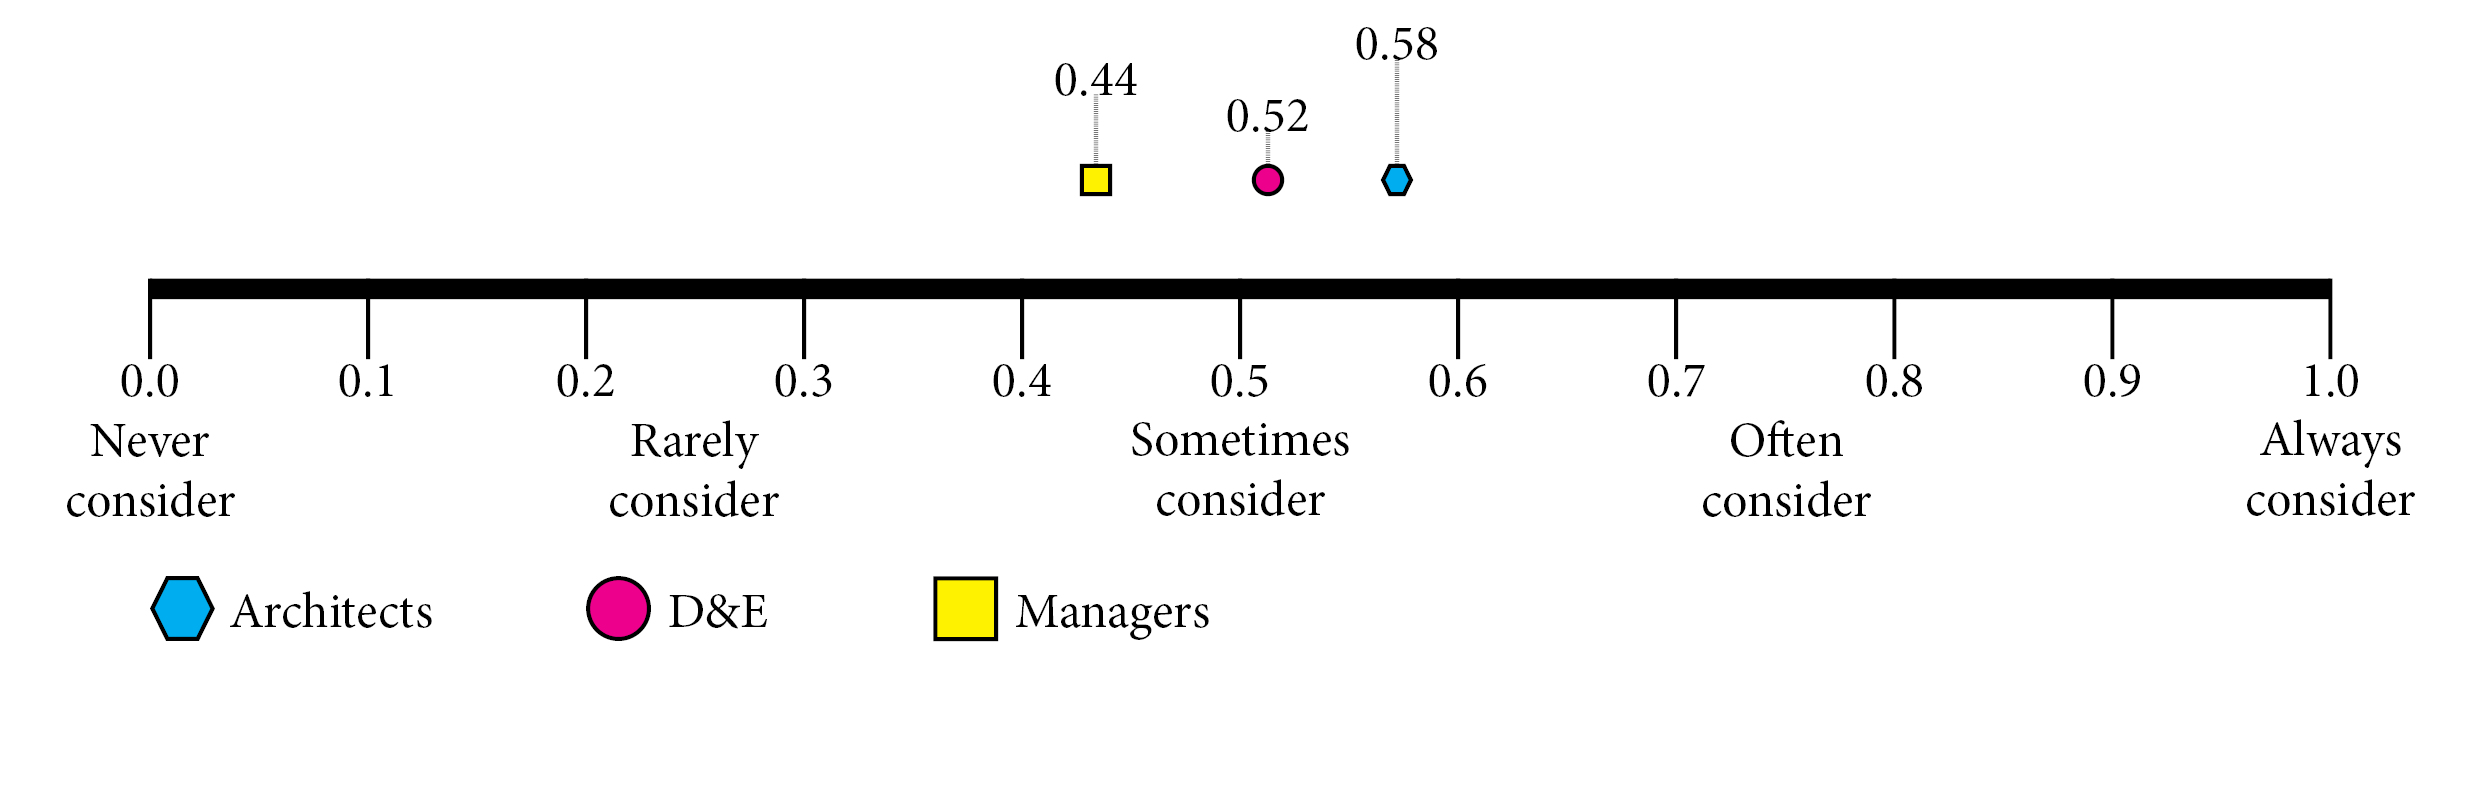
\includegraphics[width=\linewidth]{scorelines/aspect12.png}
        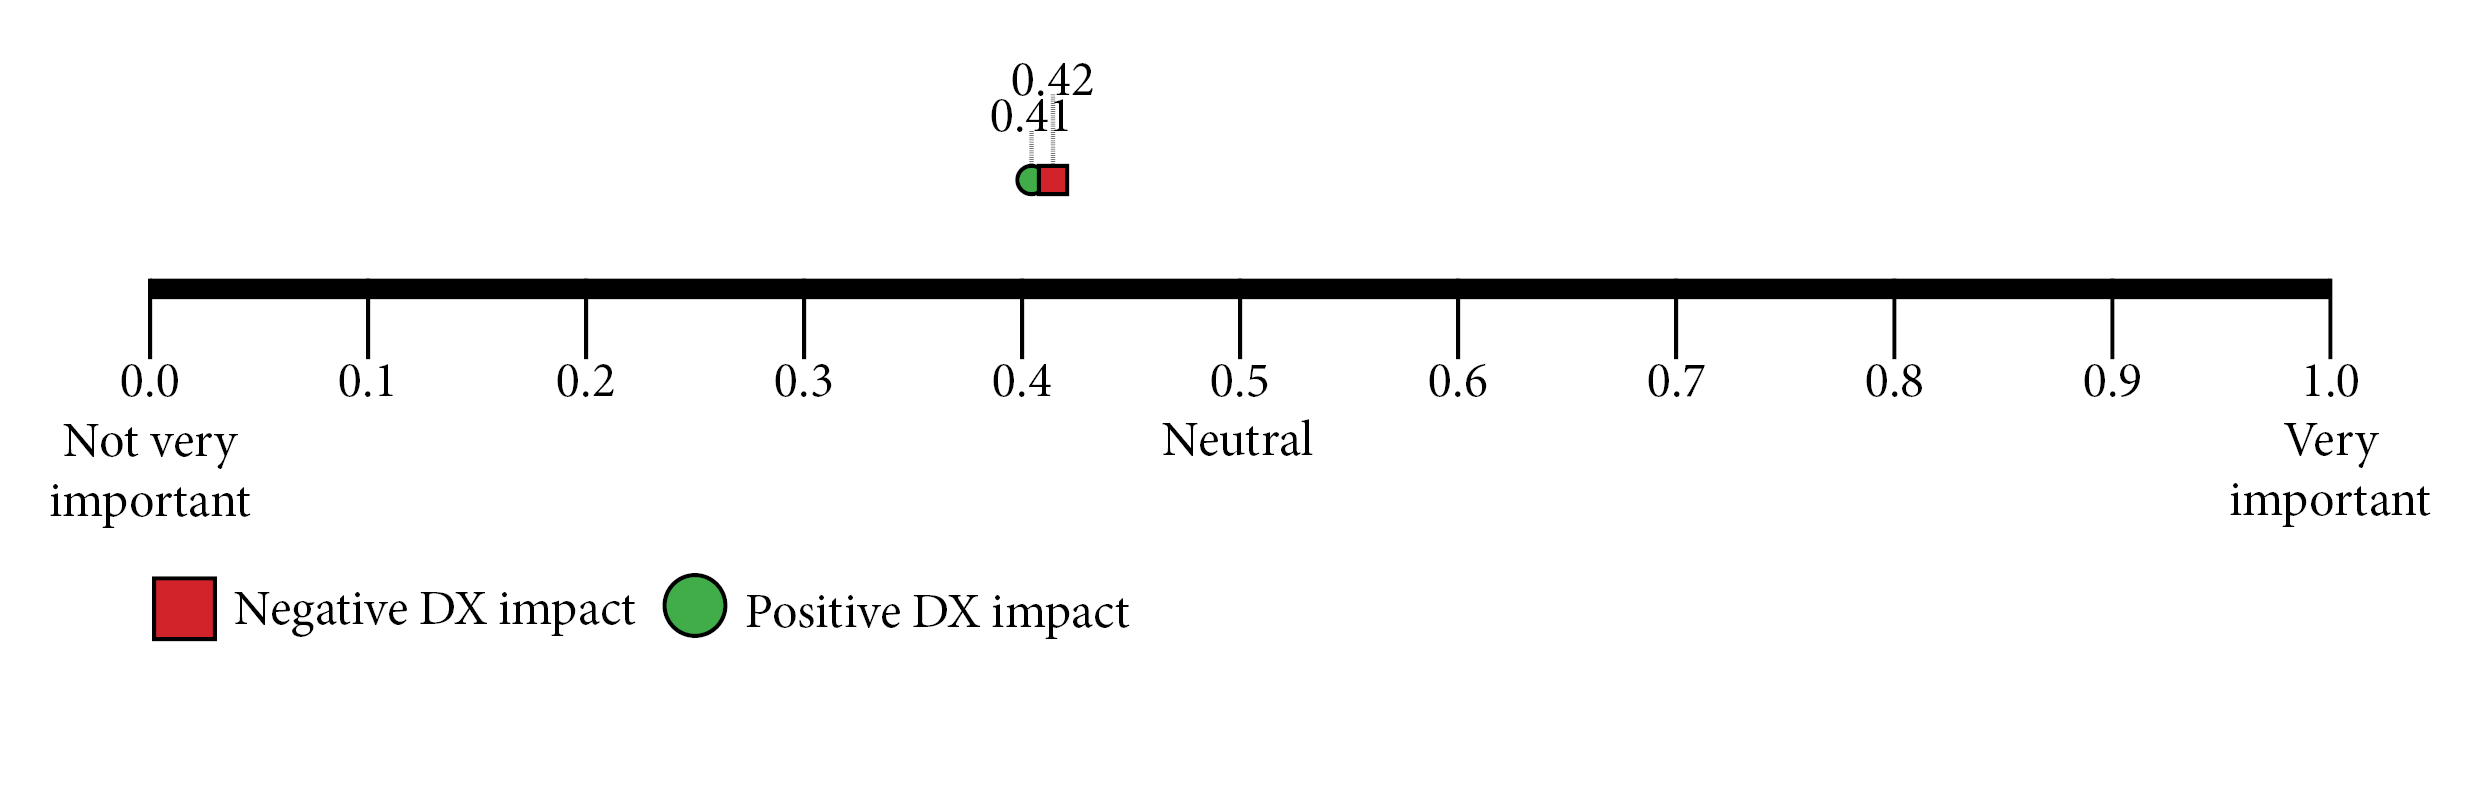
\includegraphics[width=\linewidth]{dxscorelines/dxaspect12.png}
        \caption{Scoring for "The software is compatible with different platforms"}
        \label{fig:aspect12}
    \end{figure}
    Having your software platform be compatible with many different platforms is a requirement for some users, a bonus for some. The effort to do this is however high. If you plan to implement this, make sure that the increase in potential users is worth the effort to do this. You need to be aware that is highly increases all future maintenance for your platform. As we can see in figure \ref{fig:aspect12}, it does not score very high. The recommendation is therefor to skip this aspect, if you are not sure that the increase in users is worth the effort. \\ \\
    \textbf{Verdict: Not very important. High effort, low-medium payoff.}
    
    \paragraph{The software is offered in more than one programming language}
    \begin{figure}[H]
        \centering
        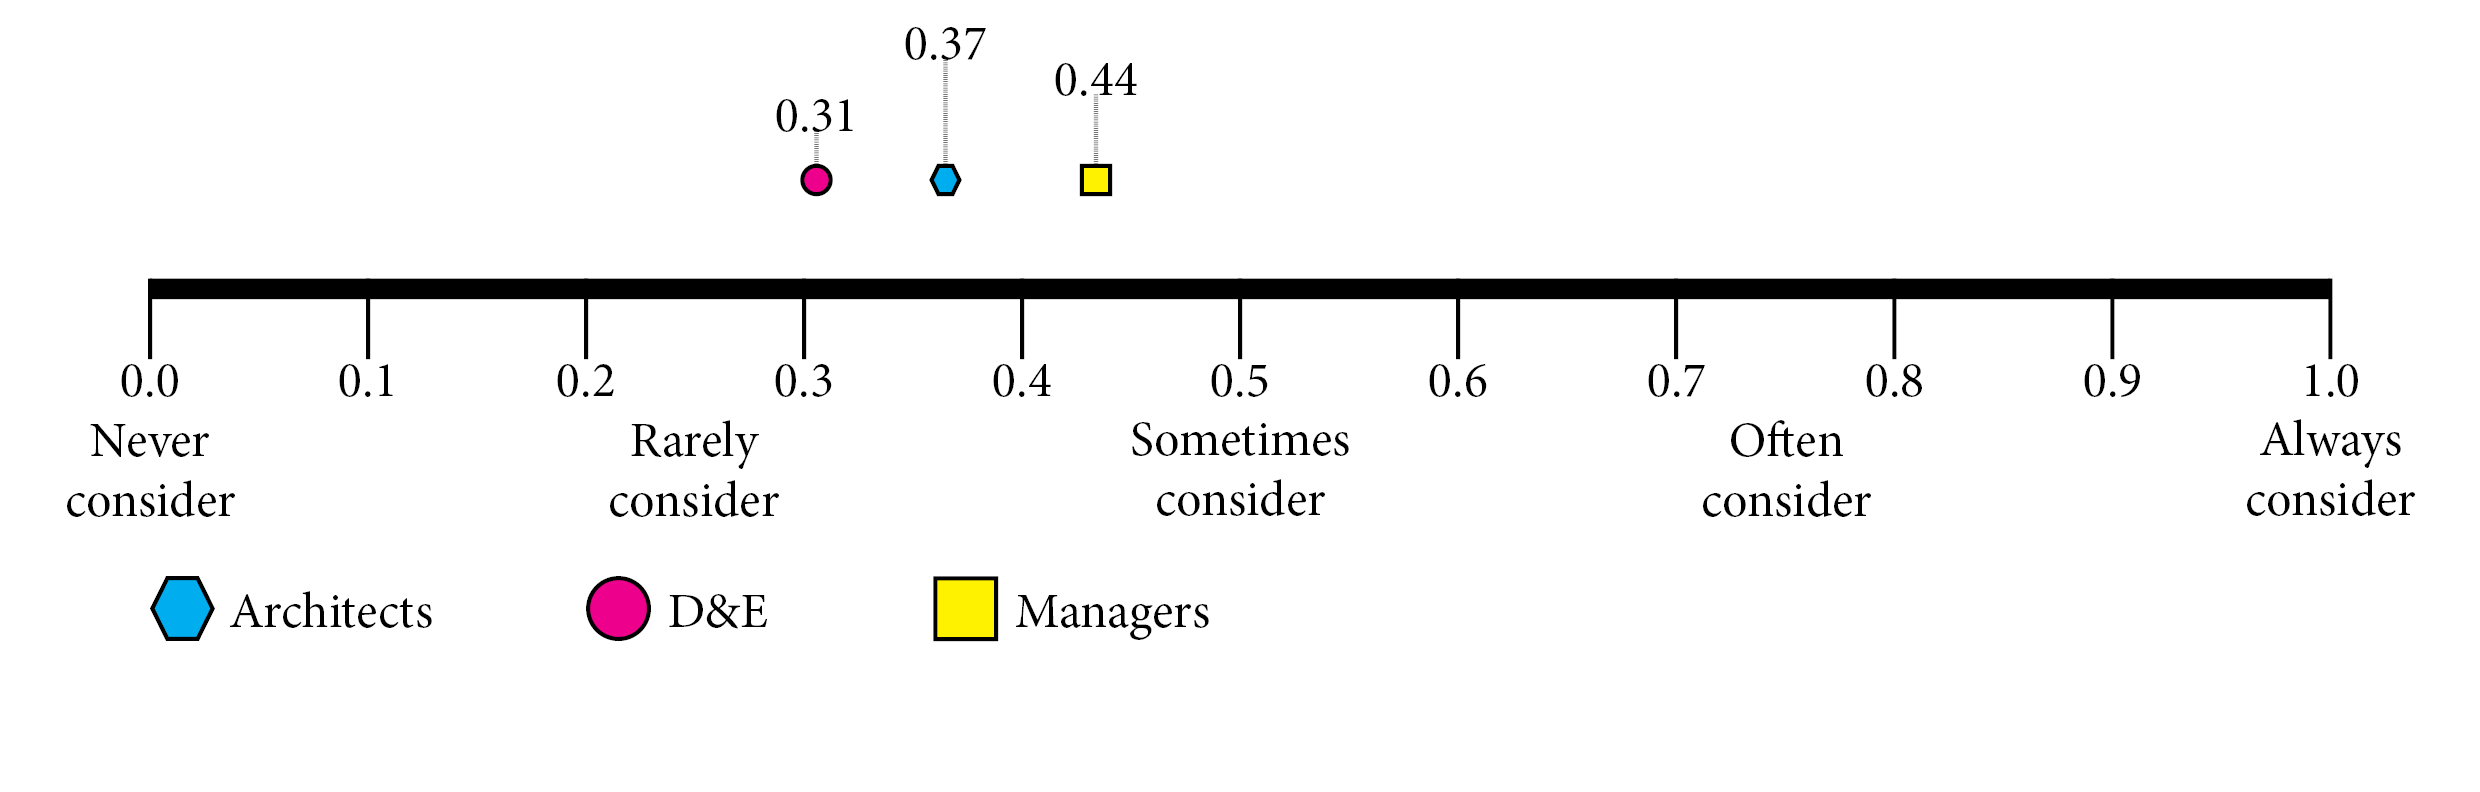
\includegraphics[width=\linewidth]{scorelines/aspect13.png}
        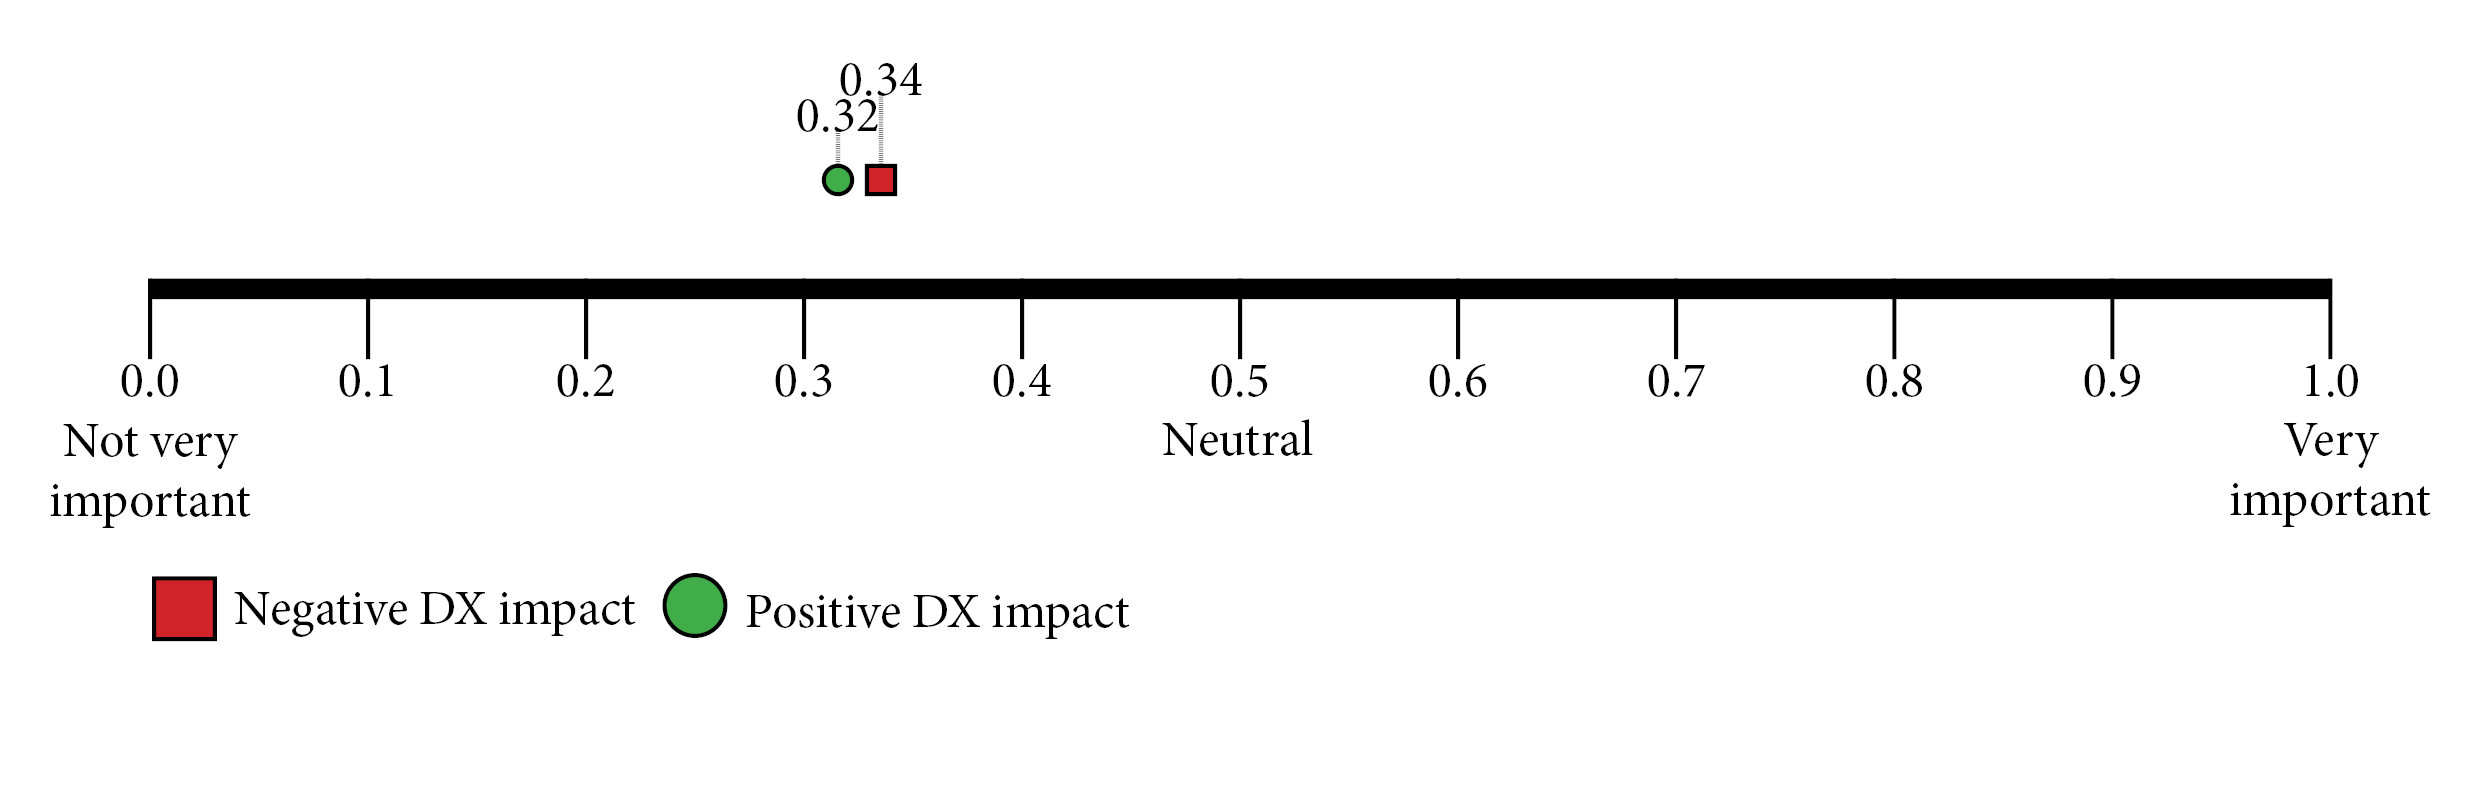
\includegraphics[width=\linewidth]{dxscorelines/dxaspect13.png}
        \caption{Scoring for "The software is offered in more than one programming language"}
        \label{fig:aspect13}
    \end{figure}
    Having your platform be compatible with more than one language takes a big effort. It takes a long time to develop and doubles the maintenance needed. As we can see in figure \ref{fig:aspect13} it's not ranked high at all. The recommendation is therefor to ignore this aspect. The effort compared with the payoff is not worth it. \\ \\
    \textbf{Verdict: Not important. High effort, low payoff.}
    
    \paragraph{The software is open source}
    \begin{figure}[H]
        \centering
        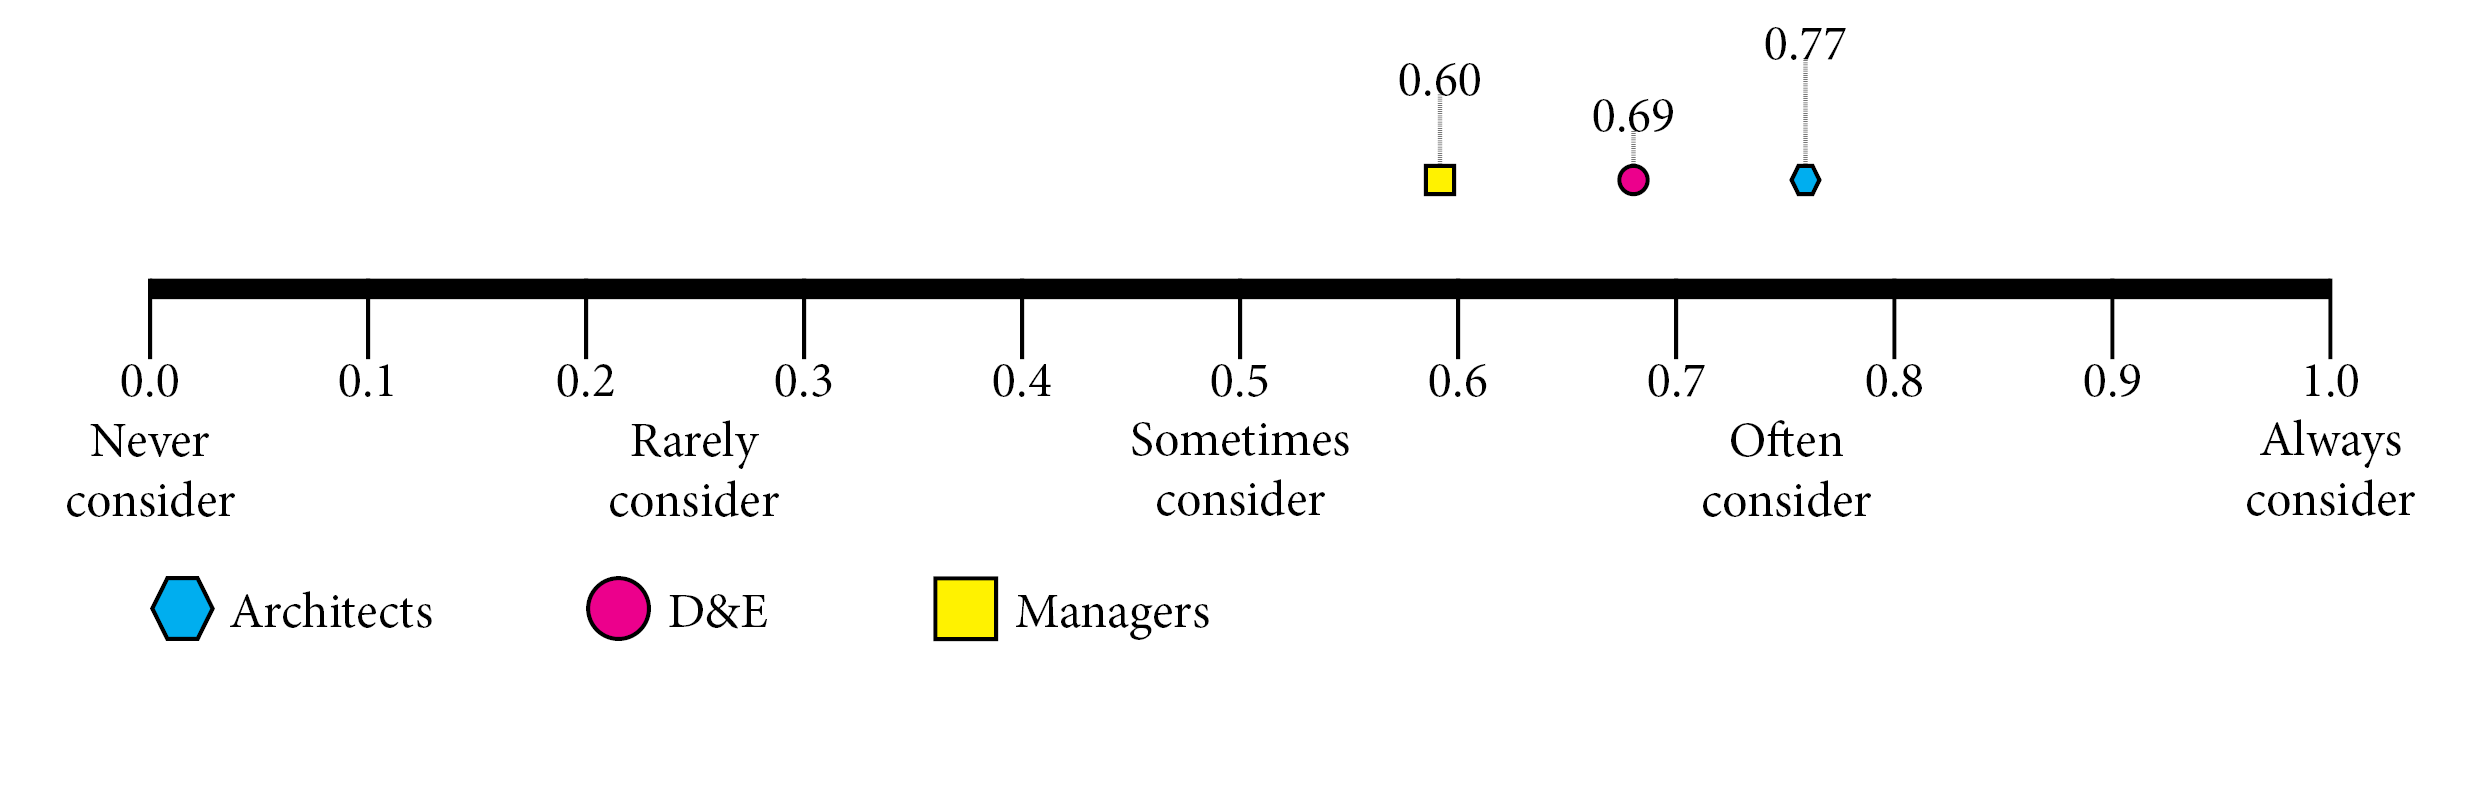
\includegraphics[width=\linewidth]{scorelines/aspect14.png}
        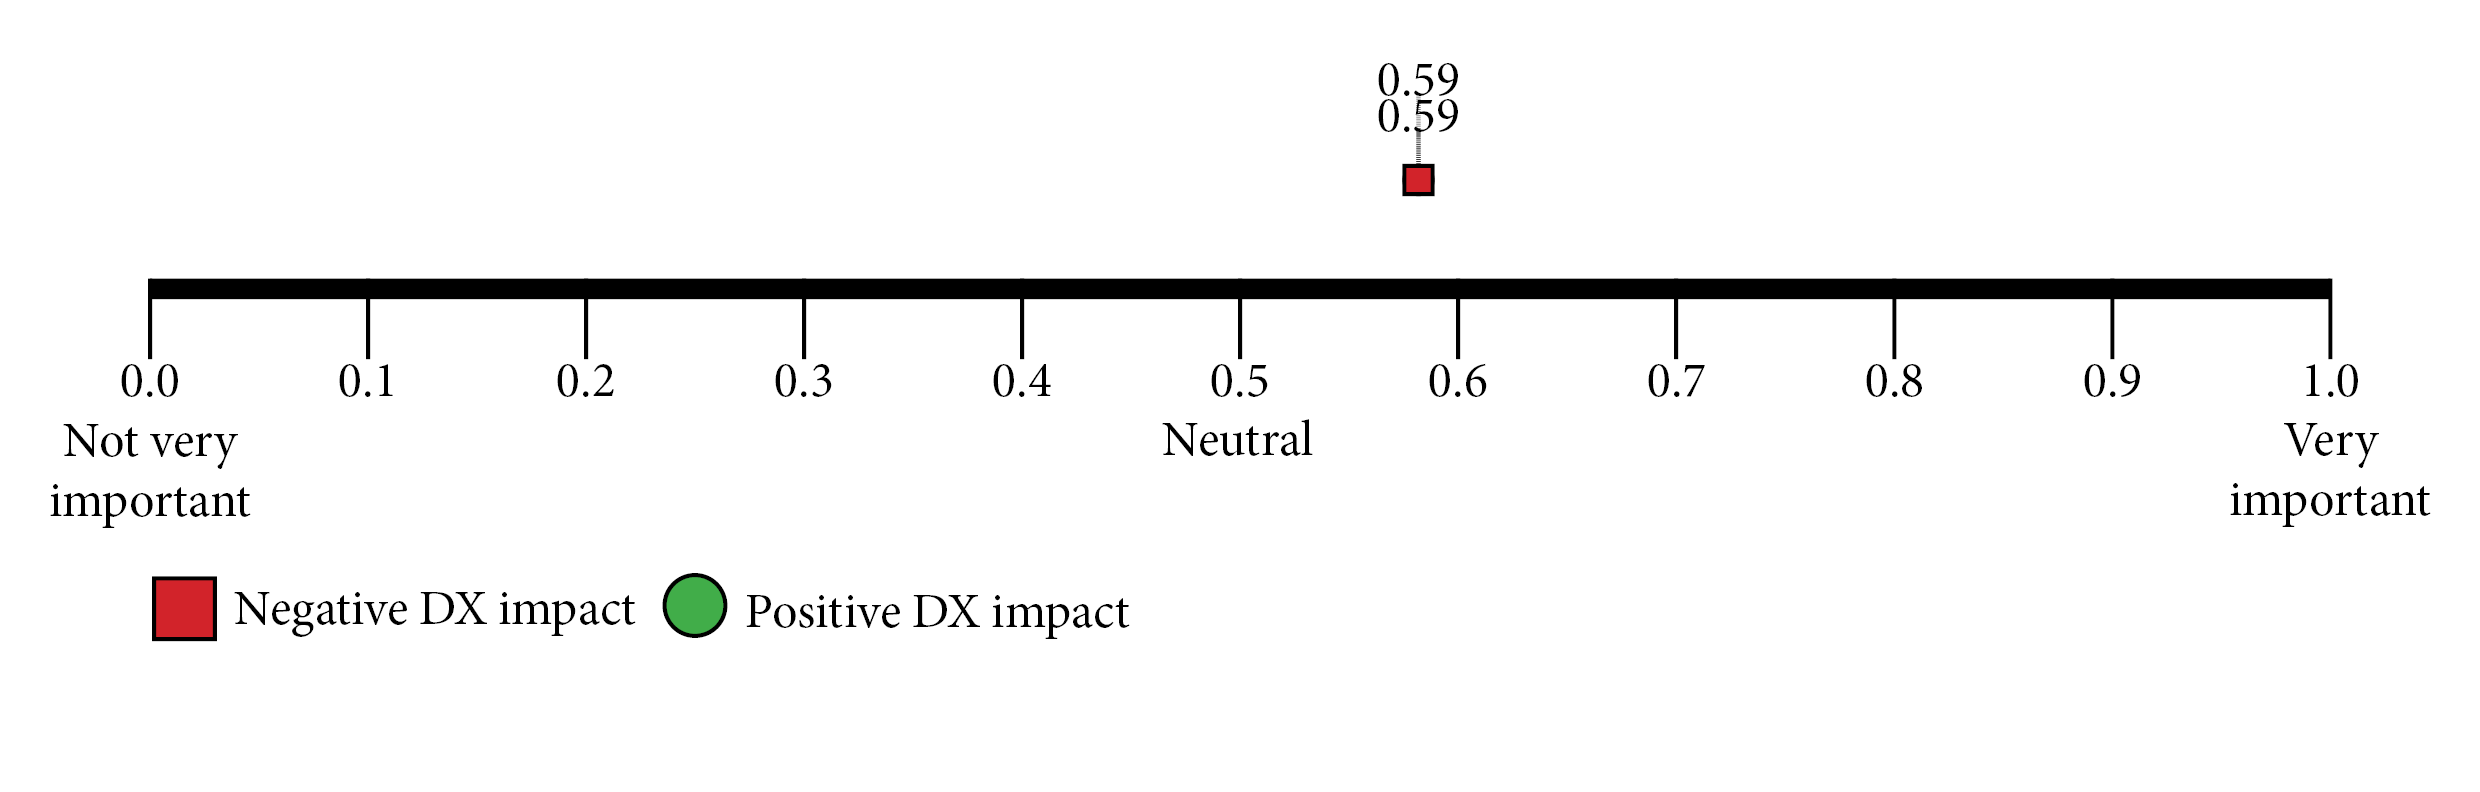
\includegraphics[width=\linewidth]{dxscorelines/dxaspect14.png}
        \caption{Scoring for "The software is open source"}
        \label{fig:aspect14}
    \end{figure}
    Being open source has both benefits and limitations. It is out of the scope of this research paper to evaluate these. But as we can see in figure \ref{fig:aspect14} it's quite important to developers and architects. The recommendation is therefor to try to be open source if you can. If it's not something that the company is used to, be aware that it requires other ways of working than conventional software that is close-source. If you decide to make an open-source software platform, make you have the expertise in the company to be able to handle this type of software. It has a potential to increase the amount of users, but if you don't use the benefits that open-source gives, it may not pay off. \\ \\
    \textbf{Verdict: Important. Medium-high effort, high payoff.}
    
    \paragraph{The software uses the programming language I am most comfortable with}
    \begin{figure}[H]
        \centering
        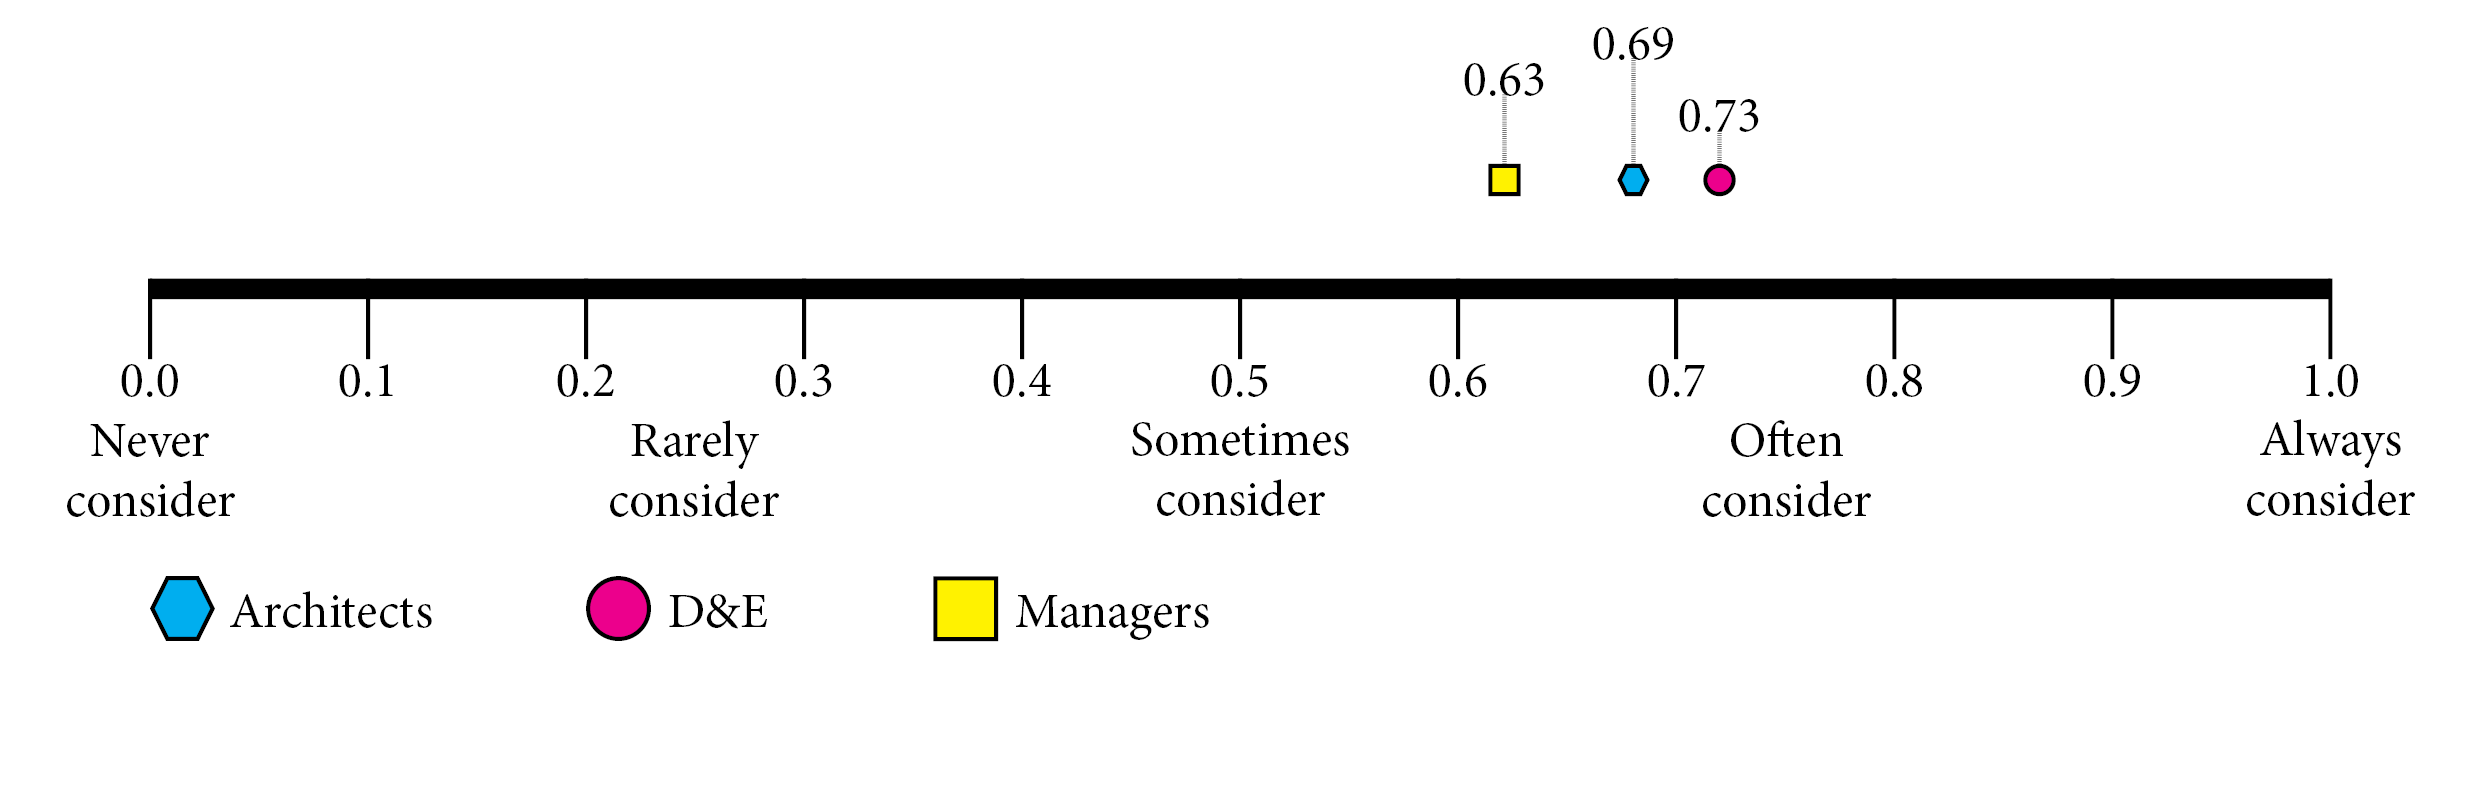
\includegraphics[width=\linewidth]{scorelines/aspect15.png}
        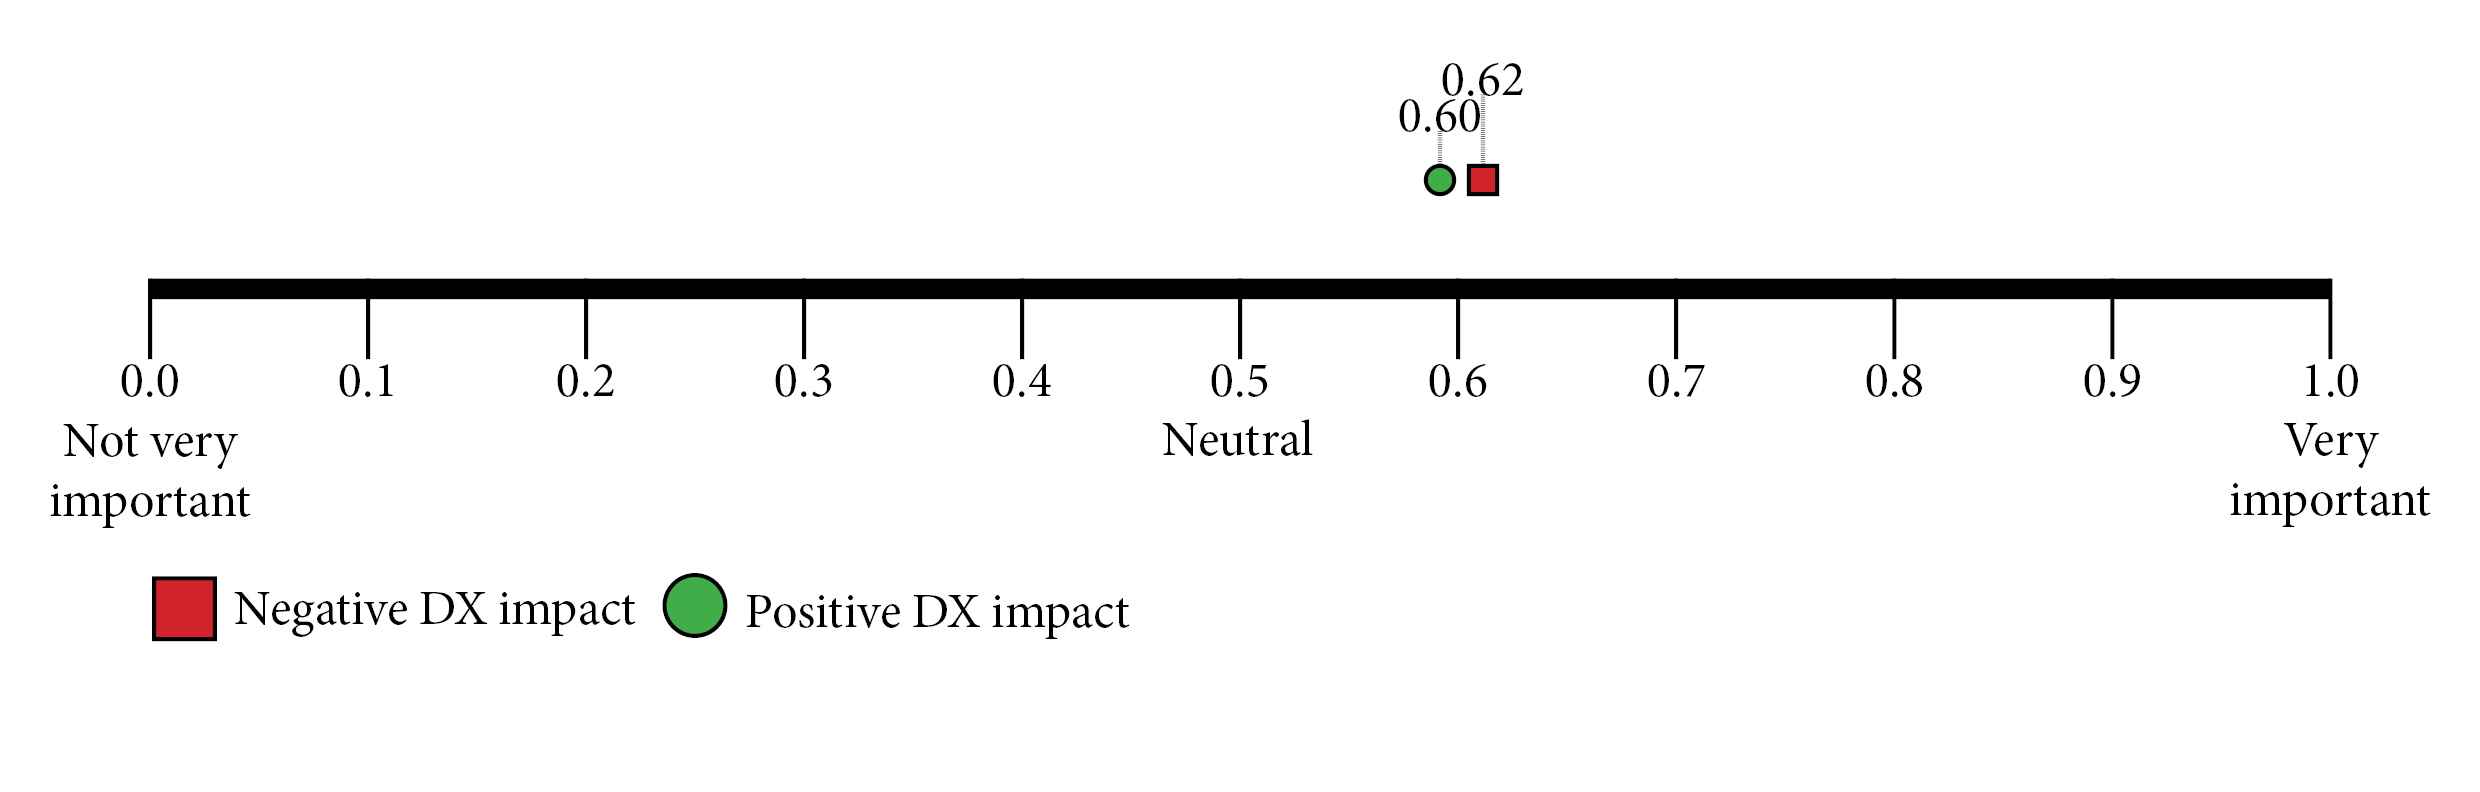
\includegraphics[width=\linewidth]{dxscorelines/dxaspect15.png}
        \caption{Scoring for "The software uses the programming language I am most comfortable with"}
        \label{fig:aspect15}
    \end{figure}
    Developers tend to be more comfortable working with certain languages, and it's unique for every person. As we can see in figure \ref{fig:aspect15} it is quite important to people that a software platform uses their favourite language. However, as stated before, providing several languages is not worth the effort. The recommendation is therefor to be attentive to what programming languages are popular, and to see how the trends change. Be aware however that these trends are just that, trends. New languages emerge all the time as "the new hot thing". The safer bet is to offer your software platform in a popular language, that is predicted to be popular for quite some time. \\ \\
    \textbf{Verdict: Important. Medium effort, high payoff.}
    
    \paragraph{There exists an active online community around the software}
    \begin{figure}[H]
        \centering
        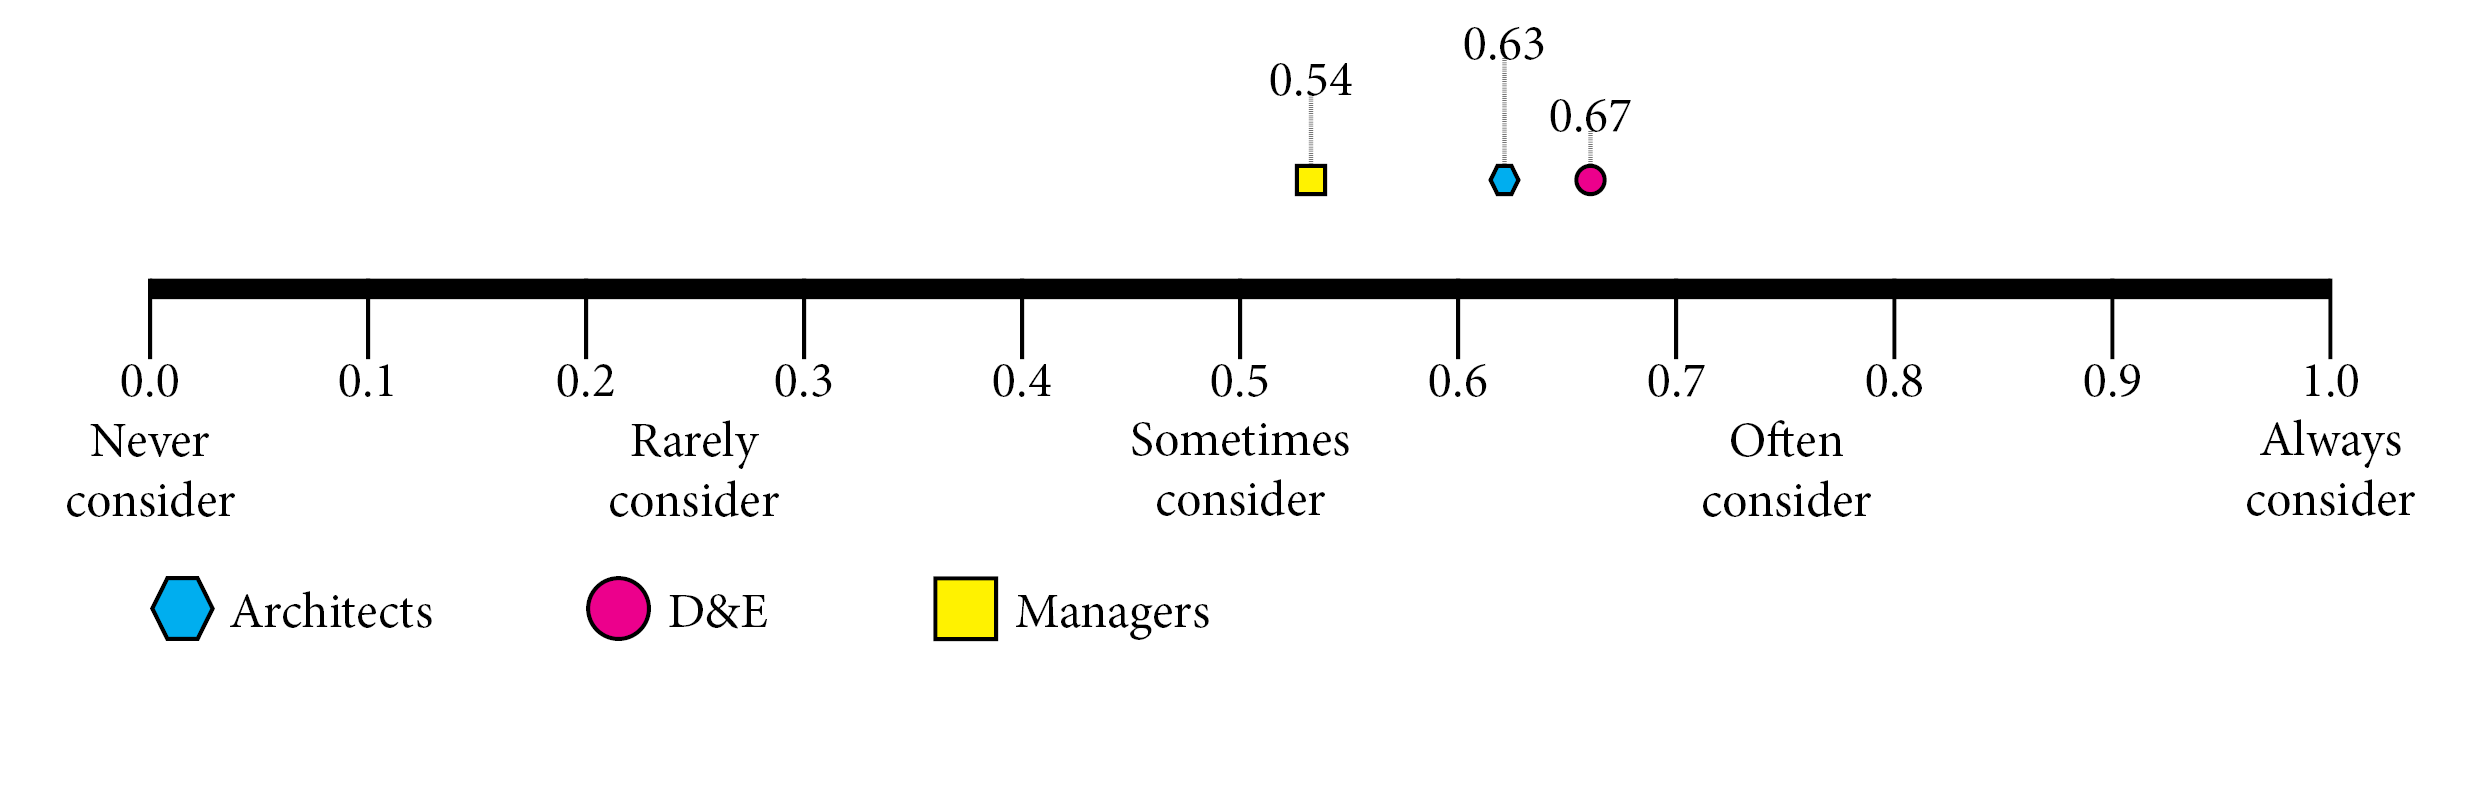
\includegraphics[width=\linewidth]{scorelines/aspect16.png}
        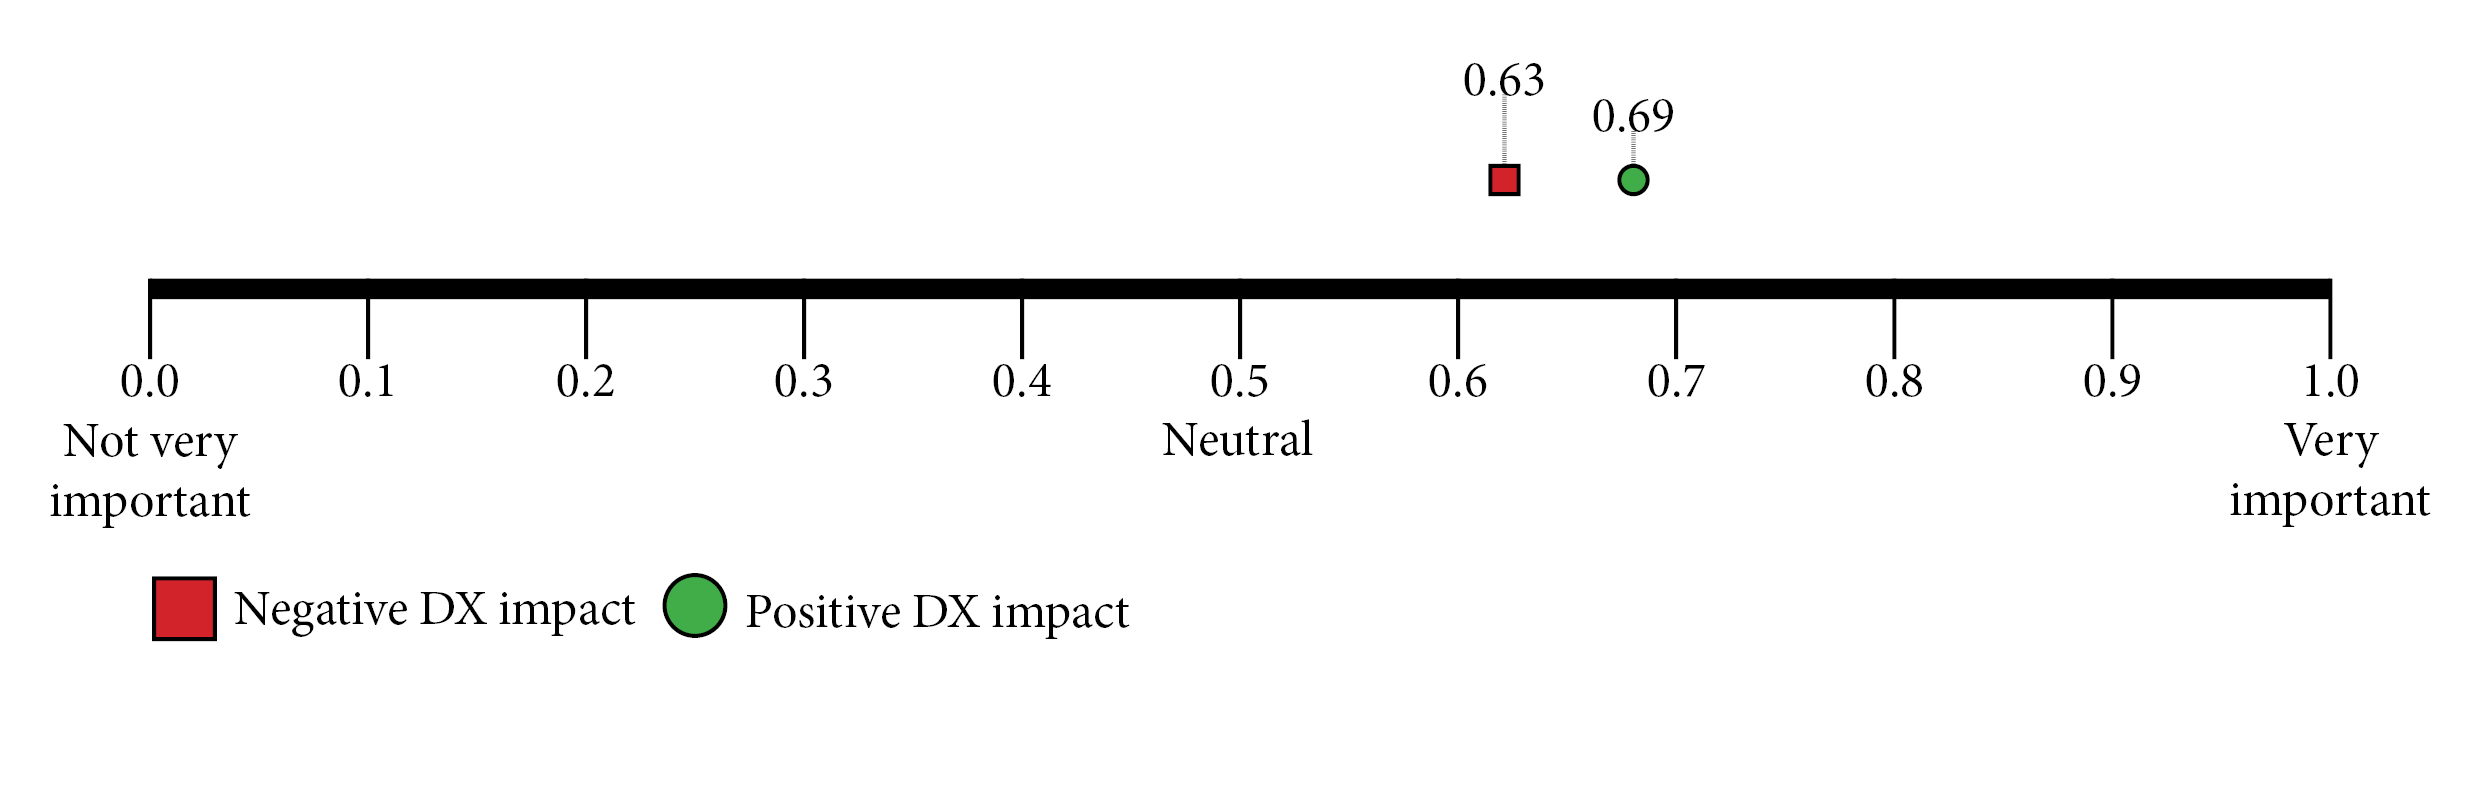
\includegraphics[width=\linewidth]{dxscorelines/dxaspect16.png}
        \caption{Scoring for "There exists an active online community around the software"}
        \label{fig:aspect16}
    \end{figure}
    It can be difficult, if not impossible, to forcefully create an online community around your software platform. It's not up to the company if people engage in online discussions, it's up to the users themselves. The company can however provide platforms for discussions. The effort to create an online forum for users to discuss doesn't have to be too big, but is a foundation to create a community. Often communities will naturally emerge on other places, such as Stack Overflow. The company can help the online community prosper by keeping an eye on these communities as well, and answer question there. This also builds a trust between the user and the company. 
    
    Online communities is primarily used for questions and answers to help out when the documentation is not enough. The effort to make sure your online community has the answers they need is somewhat big. The recommendation is to take extra care of your online community when it's new and small, and less when it's big enough that it takes care of itself. Never ignore it though, pay attention to suggestions and issues that your online community has. \\ \\
    \textbf{Verdict: Important, keep in mind. Medium effort, medium-high payoff.}